\documentclass[a4paper,12pt,twoside]{article}

% --- Codificación: agnóstica al motor ---
% pdflatex necesita inputenc + fontenc; lualatex/xelatex ya usan
% UTF-8 nativo y rompen si se carga inputenc.
\usepackage{iftex}
\ifPDFTeX
  \usepackage[utf8]{inputenc}
  \usepackage[T1]{fontenc}
\fi

% --- Paquetes básicos ---
\usepackage[spanish, es-noshorthands]{babel}
\usepackage{hyperref}
\usepackage{booktabs}
\usepackage{amsmath, amsfonts, amssymb}
\usepackage{listings}
\usepackage{graphicx}
\usepackage{subcaption}
\usepackage{tcolorbox}
\usepackage{enumitem}
\usepackage[a4paper, top=2cm, bottom=2.5cm, left=2.5cm, right=2.5cm]{geometry}
\usepackage{csquotes}
\usepackage[style=ieee, backend=biber]{biblatex}
\addbibresource{references.bib}
\usepackage{placeins}
\usepackage{tikz}
\usetikzlibrary{shapes.geometric, arrows.meta, positioning, calc, fit, backgrounds, babel}
\usepackage{pgfplots}
\pgfplotsset{compat=1.18}
\usepgfplotslibrary{statistics}
\usepackage{xcolor}
\usepackage{multirow}
\usepackage{array}
\usepackage{tabularx}
\usepackage{ragged2e}
\newcolumntype{Y}{>{\RaggedRight\arraybackslash}X}

% --- Configuración de listings para Python ---
\definecolor{codegreen}{rgb}{0,0.6,0}
\definecolor{codegray}{rgb}{0.5,0.5,0.5}
\definecolor{codepurple}{rgb}{0.58,0,0.82}
\definecolor{backcolour}{rgb}{0.97,0.97,0.97}

\lstdefinestyle{pythonstyle}{
    backgroundcolor=\color{backcolour},
    commentstyle=\color{codegreen}\itshape,
    keywordstyle=\color{blue}\bfseries,
    numberstyle=\tiny\color{codegray},
    stringstyle=\color{codepurple},
    basicstyle=\ttfamily\footnotesize,
    breakatwhitespace=false,
    breaklines=true,
    captionpos=b,
    keepspaces=true,
    numbers=left,
    numbersep=5pt,
    showspaces=false,
    showstringspaces=false,
    showtabs=false,
    tabsize=4,
    frame=single,
    rulecolor=\color{gray!40},
    language=Python
}

% --- Evitar que los floats crucen subsecciones ---
\makeatletter
\AtBeginDocument{%
  \let\origsubsection\subsection
  \renewcommand{\subsection}{\FloatBarrier\origsubsection}%
}
\makeatother

% --- Parámetros de colocación de flotantes para minimizar huecos ---
% Permitimos más flotantes por página y menos texto mínimo, así
% [t] no fuerza páginas casi vacías cuando una figura no cabe junto
% a su párrafo de referencia.
\setcounter{topnumber}{4}
\setcounter{bottomnumber}{2}
\setcounter{totalnumber}{6}
\renewcommand{\topfraction}{0.95}
\renewcommand{\bottomfraction}{0.95}
\renewcommand{\textfraction}{0.05}
\renewcommand{\floatpagefraction}{0.85}

% --- Asegurar texto justificado (por defecto en LaTeX) ---
\tolerance=1
\emergencystretch=\maxdimen
\hyphenpenalty=10000
\hbadness=10000

% --- Redefinir \cleardoublepage para que las páginas en blanco no lleven número ---
\makeatletter
\def\cleardoublepage{\clearpage\if@twoside \ifodd\c@page\else
    \thispagestyle{empty}%
    \hbox{}\newpage\if@twocolumn\hbox{}\newpage\fi\fi\fi}
\makeatother

% --- Comando para páginas en blanco sin numeración ---
\newcommand{\blankpage}{%
    \newpage
    \thispagestyle{empty}
    \mbox{}
    \newpage
}

\title{\Huge \textbf{Práctica Final: Sistema Multiagente Financiero con LangGraph, FastAPI y Observabilidad Humana}}
\author{Diego Esclarín \and Sofía Contreras}
\date{\today}

\begin{document}

% --- Página 1: Portada (Interna -1) ---
\begin{titlepage}
    \thispagestyle{empty}
    \centering
    \vspace*{1cm}

    {\Huge \textbf{Práctica Final: Sistema Multiagente Financiero con LangGraph, FastAPI y Observabilidad Humana} \par}
    \vspace{1.5cm}

    \begin{figure}[h]
        \centering
        
\includegraphics[width=0.6\textwidth]{figures/Logo_URJC.png}
    \end{figure}

    \vfill

    {\large \textbf{Autores:} \par}
    \vspace{0.3cm}
    {\large Diego Esclarín (51729611N) \par}
    {\large Sofía Contreras (09848471D) \par}

    \vspace{1.5cm}

    {\large Aprendizaje en Inteligencia Artificial \par}
    {\large Grado en Ingeniería en Inteligencia Artificial \par}
    {\large Universidad Rey Juan Carlos \par}
    {\large Curso 2025--26 \par}

\end{titlepage}
\setcounter{page}{0}

% --- Página 2: Blanco (Interna 0) ---
\blankpage

% --- Índices ---
\thispagestyle{empty}
\tableofcontents
\cleardoublepage

\thispagestyle{empty}
\listoffigures
\cleardoublepage

\thispagestyle{empty}
\listoftables
\cleardoublepage

% --- Inicio del contenido ---
\pagestyle{plain}

\section{Introducción}
\label{sec:introduccion}

La memoria documenta el desarrollo de la práctica final de la
asignatura \textit{Aprendizaje en Inteligencia Artificial} del Grado en
Ingeniería en Inteligencia Artificial de la Universidad Rey Juan Carlos.
El proyecto, denominado internamente \textbf{PFINAL\_AP-IA}, constituye
la finalización e integración de las seis prácticas anteriores
(P1--P5) bajo un único sistema multiagente conversacional dedicado a la
gestión financiera personal.

El sistema toma la forma de un asistente financiero capaz de mantener
un diálogo natural con el usuario, registrar transacciones a partir de
texto o imágenes (OCR), detectar anomalías de gasto, generar
predicciones temporales, autenticar mediante biometría facial y
explicar sus respuestas mediante visualizaciones dinámicas. La
arquitectura se apoya en \textbf{LangGraph}~\cite{langgraph} para la
orquestación de agentes, \textbf{FastAPI}~\cite{fastapi} para exponer
cada módulo como microservicio REST, \textbf{Next.js}~\cite{nextjs}
en el frontend y \textbf{Langfuse}~\cite{langfuse} para la
monitorización de trazas, llamadas a herramientas, latencias y
consumo de tokens.

El documento se estructura en cinco capítulos. El capítulo de
\textit{Contexto} sitúa la práctica dentro del recorrido de las prácticas anteriores y
recoge los requisitos funcionales. El \textit{Estado del arte} repasa
los frameworks y técnicas que sustentan las decisiones de diseño. La
\textit{Propuesta} detalla la arquitectura implementada, los dos roles
diferenciados (usuario y administrador), la memoria conversacional, la
distribución de los módulos P1--P5 como microservicios, la evolución
incremental sobre P2, P3 y P5, las metodologías de prompt engineering
empleadas y la estrategia de pruebas unitarias y de estrés. Las
\textit{Conclusiones} resumen los resultados cuantitativos obtenidos y
las líneas de trabajo futuro.

\cleardoublepage

\section{Contexto}
\label{sec:contexto}

\subsection{Integración de P1--P5}

A lo largo de la asignatura se han implementado cinco prácticas
independientes pero complementarias, cada una orientada a un eje
distinto del aprendizaje automático aplicado al dominio financiero
personal:

\begin{itemize}[leftmargin=1.5em,itemsep=0.2em]
  \item \textbf{P1 --- Predicción temporal.} Modelos de regresión y
        series temporales (Random Forest, HistGradientBoosting y
        ARIMA) para anticipar el gasto del mes siguiente.
  \item \textbf{P2 --- Clasificación multietiqueta.} Asignación de la
        categoría (\textit{Area}) a una transacción a partir de su
        descripción textual mediante un \texttt{SGDClassifier} sobre
        char $n$-gramas.
  \item \textbf{P3 --- OCR financiero.} Extracción del importe total
        de facturas reales mediante \texttt{PaddleOCR} y un scorer
        basado en Gradient Boosting.
  \item \textbf{P4 --- Agente conversacional.} Primer contacto con
        \texttt{LangGraph} y la orquestación de herramientas mediante
        LLM.
  \item \textbf{P5 --- Biometría facial y detección de anomalías.}
        Pipeline MTCNN + FaceNet + DenseNet201 para autenticación
        biométrica con \textit{liveness}, e \texttt{IsolationForest}
        para anomalías financieras.
\end{itemize}

La práctica final exige evolucionar la práctica 6, que integra las cinco anteriores bajo un único sistema
multiagente que conserva la fiabilidad de las soluciones individuales
ganando cohesión, persistencia multiusuario y observabilidad
profesional. El enunciado considera P4 cubierto, por lo
que la \textit{evolución incremental} (Sección~\ref{subsec:evoluciones})
recae sobre P2, P3 y P5.

\subsection{Requisitos funcionales}

La especificación de la práctica final incluye un conjunto de
requisitos transversales que el sistema debe satisfacer. La
Tabla~\ref{tab:requisitos} los enumera y los enlaza con la sección de
la propuesta en la que se justifica su cumplimiento.

\begin{table}[!htbp]
  \centering
  \footnotesize
  \begin{tabularx}{\linewidth}{@{}p{0.42\linewidth} X@{}}
    \toprule
    \textbf{Requisito} & \textbf{Sección de la propuesta} \\
    \midrule
    Histórico conversacional para el LLM &
      \S\ref{subsec:memoria-conversacional} \\
    Recuperación de chats previos &
      \S\ref{subsec:memoria-conversacional} \\
    Diagramas visuales dinámicos (XAI) &
      \S\ref{subsec:xai-visualizacion} \\
    Monitorización del sistema (MonitorAgent) &
      \S\ref{subsec:monitorizacion} \\
    Al menos dos roles diferenciados en LangGraph &
      \S\ref{subsec:roles} \\
    Módulos P1--P5 distribuidos vía API REST &
      \S\ref{subsec:microservicios} \\
    Diálogo natural con detección de intención &
      \S\ref{subsec:intencion} \\
    Uso de Langfuse &
      \S\ref{subsec:langfuse} \\
    Prompt engineering (ASPECCT) &
      \S\ref{subsec:aspect} \\
    Tres evoluciones incrementales (P2, P3, P5) &
      \S\ref{subsec:evoluciones} \\
    Evaluaciones cuantitativas &
      \S\ref{subsec:evoluciones} \\
    Pruebas unitarias y de estrés &
      \S\ref{subsec:tests} \\
    \bottomrule
  \end{tabularx}
  \caption{Mapeo entre los requisitos del enunciado y las secciones de la
  propuesta.}
  \label{tab:requisitos}
\end{table}

\subsection{Restricciones técnicas y de despliegue}

El sistema se ha diseñado con tres restricciones operativas
relevantes que han condicionado tanto la elección de tecnologías
como la arquitectura final.

\paragraph{Stack gratuito o de coste mínimo.} El LLM principal corre
en \textit{Groq Cloud} (plan gratuito con \textit{rate limits} de
30 \textit{requests}/min para \texttt{llama-3.3-70b-versatile}), la
base de datos vive en \textit{Supabase} (Postgres gestionado con
500\,MB en el plan \textit{free}), la observabilidad en
\textit{Langfuse Cloud} (50.000 \textit{traces}/mes gratuitos) y el
frontend en \textit{Vercel}. El \textit{backend} se sirve localmente
con \texttt{uvicorn} y se expone públicamente vía un túnel
\textit{ngrok} con dominio estático, ya que el plan gratuito de
Vercel no permite contenedores con dependencias nativas pesadas
(PaddlePaddle, PyTorch, OpenCV) en sus \textit{serverless functions}.

\paragraph{Compatibilidad de versiones.} \texttt{PaddleOCR 2.6.2}
exige \texttt{numpy<2.0}, lo que ancla todo el \textit{stack} a
\texttt{NumPy 1.26.4}. Esta restricción ha condicionado la elección del
resto de dependencias: \texttt{scikit-learn 1.5.0},
\texttt{torch 2.5.1}, \texttt{langgraph 1.x},
\texttt{facenet-pytorch} (en lugar de \texttt{deepface}, que arrastra
TensorFlow). El \textit{trade-off} aceptado es no poder usar
\texttt{numpy 2.x} ni las versiones más recientes de
\texttt{scikit-learn}; a cambio, todo el \textit{stack} convive en
un único \textit{entry point} (\texttt{uvicorn}) sin necesidad de
aislar P3 en un microservicio aparte.

\paragraph{Activos pesados con Git LFS.} Los modelos preentrenados
(\texttt{models/area\_classifier.joblib},
\texttt{models/ocr\_total\_extractor.joblib} y
\texttt{models/liveness\_kaggle.pth}, $\sim$78\,MB en total) viajan
por \textit{Git Large File Storage} para no inflar el historial del
repositorio. Sin habilitar \texttt{git lfs install} antes del
\texttt{clone}, los modelos se descargan como punteros de 134 bytes
y el \textit{backend} falla al cargar el clasificador de
\texttt{Area} en el primer turno. Adicionalmente, las dependencias
DL (PaddleOCR, PyTorch, MediaPipe) ocupan $\sim$2{,}5\,GB en
\texttt{.venv}, lo que descarta la idea inicial de empaquetar la
aplicación en una imagen Docker desplegable en plataformas
\textit{serverless} sin almacenamiento persistente.

\paragraph{Cumplimiento RGPD y aislamiento multiusuario.} El sistema
maneja datos personales sensibles (transacciones financieras y
\textit{embeddings} biométricos), por lo que el cumplimiento del
Reglamento General de Protección de Datos no es una característica
opcional sino una restricción de diseño. Esto se traduce en cuatro
exigencias concretas: (i) los \textit{embeddings} faciales se
almacenan cifrados en disco con \texttt{Fernet} (AES-128) sobre una
clave derivada con \texttt{PBKDF2-HMAC-SHA256} a 310.000 iteraciones,
nunca en claro; (ii) las contraseñas se almacenan con \texttt{bcrypt}
(\textit{cost factor} 12) sin recurrir a \texttt{passlib} ---
incompatible con \texttt{bcrypt 4.x}; (iii) las notificaciones a
Telegram nunca exponen importes ni descripciones salvo que el
usuario active \texttt{notification\_level='full'}; y (iv) la
detección de anomalías nunca compara las transacciones de un usuario
contra el histórico de otro.

\cleardoublepage

\section{Estado del Arte}
\label{sec:estado-arte}

Esta sección revisa los marcos teóricos y las herramientas en las que
se apoya el sistema, distinguiendo aquellas que han sido finalmente
adoptadas de las alternativas evaluadas y descartadas.

\subsection{Orquestación de agentes con LangGraph}

LangGraph~\cite{langgraph} (LangChain Labs) es una biblioteca para
construir sistemas multiagente como grafos dirigidos cuyos nodos son
funciones Python y cuyas aristas pueden ser condicionales,
ejecutadas en función del estado tipado del grafo. Frente a
alternativas como \texttt{AutoGen} (Microsoft) o \texttt{CrewAI},
LangGraph destaca por:

\begin{itemize}[leftmargin=1.5em,itemsep=0.2em]
  \item Su \textbf{enfoque grafo + estado tipado}, que permite
        razonar formalmente sobre la trayectoria del control y
        garantiza la \textit{terminación} (en este proyecto se
        impone un \textit{iteration limit} de seis pasos).
  \item Su \textbf{soporte nativo de checkpointers} (\texttt{MemorySaver},
        \texttt{PostgresSaver}, \texttt{SqliteSaver}), que guarda
        el histórico conversacional dentro del mismo grafo sin
        necesidad de un sistema externo.
  \item La posibilidad de combinar \textit{structured output}
        (Pydantic) con LLM \textit{plain} en distintos nodos del
        mismo grafo. En el sistema se aprovecha para separar
        \textit{routing} (decisión) y \textit{narración} (texto
        natural).
\end{itemize}

\subsection{LLM y \textit{providers}}

El catálogo de proveedores ha quedado configurable por usuario, con
soporte nativo para Groq~\cite{groq}, OpenAI, Anthropic y Google. El
modelo por defecto es \texttt{llama-3.3-70b-versatile} servido por
Groq, que ofrece latencias inferiores a 500\,ms en \textit{tool
calling} gracias a su hardware LPU dedicado. Para tareas de
\textit{small-talk} y resumen rodante se usa
\texttt{llama-3.1-8b-instant}, que reduce el gasto de tokens en
operaciones poco exigentes.

\subsection{Visión por computador: OCR y biometría}

Para OCR se adoptó \texttt{PaddleOCR}~\cite{paddleocr} (versión 2.6.2)
por su rendimiento sobre texto en castellano y su capacidad de
funcionar en CPU sin GPU externa, descartando \texttt{EasyOCR} (menor
precisión sobre tickets en euros). Para biometría se eligió
\texttt{facenet-pytorch}~\cite{facenet} (\texttt{InceptionResnetV1}
pre-entrenado en VGGFace2) en lugar de \texttt{deepface}/\texttt{ArcFace},
evitando así introducir TensorFlow en el stack. La detección de rostros se apoya en
\texttt{MTCNN}~\cite{mtcnn} y la detección de vida (\textit{liveness})
en \texttt{DenseNet201}~\cite{densenet} con pesos ImageNet, completada
con un módulo \textit{anti-spoofing} basado en LBP, análisis de espacio
de color HSV/YCrCb y análisis frecuencial (FFT) para detectar
patrones Moiré de pantallas LCD. Los \textit{landmarks} faciales
necesarios para el \textit{challenge-response} de parpadeo se extraen
con \texttt{MediaPipe Face Mesh}~\cite{mediapipe}.

\subsection{Detección de anomalías y predicción temporal}

El detector de anomalías financieras combina
\texttt{IsolationForest}~\cite{isolation_forest} de
\texttt{scikit-learn} con una regla heurística de 3-sigma sobre los
importes históricos del usuario. Esta combinación, ya validada en P5,
se ha mantenido por su robustez y por la interpretabilidad de la
regla 3-sigma frente al usuario final. Para la predicción mensual
conviven tres modelos --- Random Forest, HistGradientBoosting y ARIMA
--- accesibles vía un único endpoint REST que permite seleccionar el
método.

\subsection{Clasificación de texto financiero}

Para clasificar la \texttt{Area} de una transacción se ha evolucionado
del \texttt{SGDClassifier} sobre TF-IDF de char $n$-gramas (P2
original) hacia un pipeline híbrido basado en
\textit{Sentence-BERT}~\cite{sentence_bert} con embeddings
multilingües. Este enfoque permite generalizar a descripciones que
no aparecieron en el entrenamiento (\textit{cold-start} y nuevos
idiomas) sin perder el \textit{macro-F1} en el conjunto de
entrenamiento.

\subsection{Observabilidad: Langfuse}

\texttt{Langfuse}~\cite{langfuse} (versión 3) es una plataforma de
observabilidad específica para LLM con instrumentación nativa de
LangChain/LangGraph mediante \texttt{CallbackHandler}. Recoge
automáticamente la cadena de llamadas (\textit{traces}), prompt
completo, respuesta cruda, \textit{tool calls}, latencias y consumo
de tokens. Frente a alternativas como \texttt{LangSmith} (de pago),
\texttt{Helicone} (no LangChain-native) o \texttt{Phoenix} (Arize),
Langfuse ofrece un plan gratuito generoso y un \textit{dashboard} web
suficiente para auditar la ejecución de los agentes en tiempo real.

\subsection{Prompt engineering: ASPECCT vs TAREA}

El enunciado permite escoger entre dos metodologías estructuradas de
\textit{prompting}. ASPECCT~\cite{aspect} (Audience, Style, Purpose,
Examples, Constraints, Context, Tone) separa \textit{style} y
\textit{tone}, lo que en el sistema permite inyectar el bloque de
estilo dependiente del rol del usuario
(\texttt{basic}/\texttt{advanced}) como un \texttt{SystemMessage}
independiente sin tocar el prompt principal. TAREA (Tarea, Audiencia,
Recursos, Estructura, Activación) resulta más compacta pero no separa
estilo y tono. Por esta razón se ha adoptado ASPECCT como metodología
oficial del proyecto.

\subsection{Pruebas de carga: Locust}

Para validar el comportamiento del sistema bajo concurrencia se ha
optado por \texttt{Locust}~\cite{locust}, un \textit{framework} de
\textit{load testing} en Python que permite describir el
comportamiento de los usuarios virtuales como clases con \texttt{@task}.
La principal ventaja sobre alternativas como JMeter o k6 es que los
escenarios se escriben en el mismo lenguaje del backend, lo que
facilita la generación de cargas realistas (registro con
\textit{multipart}, JWT, etc.) sin duplicar lógica.

\cleardoublepage

\section{Propuesta}
\label{sec:propuesta}

Esta sección describe la solución implementada, organizada en torno a
los doce requisitos del enunciado.

\subsection{Arquitectura general}
\label{subsec:arquitectura}

El sistema sigue una arquitectura en tres capas. La capa de
\textbf{presentación} la conforma un frontend en Next.js 14 (App
Router) desplegado en Vercel, con dos dominios funcionales separados:
\texttt{/chat} (financiero, usuario regular) y \texttt{/admin/chat}
(operativo, administrador). La capa de \textbf{aplicación} es una
API FastAPI servida por Uvicorn, que expone tanto los endpoints de
chat como los microservicios de los módulos \texttt{/modules/p1}
hasta \texttt{/modules/p5}. La capa de \textbf{datos} la forman una
base de datos PostgreSQL alojada en Supabase~\cite{supabase} y un
\textit{store} cifrado en disco para los \textit{embeddings}
biométricos. La Figura~\ref{fig:topology} resume esta topología.

\begin{figure}[t]
    \centering
    \begin{tikzpicture}[
    node distance=1.1cm and 1.4cm,
    every node/.style={font=\small},
    box/.style={rectangle, draw, rounded corners, minimum width=2.6cm, minimum height=0.9cm, align=center, fill=blue!8},
    orchbox/.style={rectangle, draw, rounded corners, minimum width=3.6cm, minimum height=1cm, align=center, fill=orange!15},
    dbbox/.style={cylinder, shape border rotate=90, aspect=0.25, draw, minimum width=3cm, minimum height=1.2cm, align=center, fill=green!10},
    user/.style={ellipse, draw, minimum width=2.2cm, fill=gray!10},
    arrow/.style={-Latex, thick}
]
    \node[user] (usuario) {Usuario};
    \node[orchbox, below=of usuario] (orch) {Orchestrator\\\scriptsize{(LLM: route + narrate)}};
    \node[box, below left=1.2cm and 0.3cm of orch] (sec) {Security\\\scriptsize{anomalías + biometría}};
    \node[box, below=of orch] (reg) {Registrar\\\scriptsize{manual + OCR + clf}};
    \node[box, below right=1.2cm and 0.3cm of orch] (ana) {Analyst\\\scriptsize{8 ops + forecast}};
    \node[dbbox, below=1.2cm of reg] (db) {PostgreSQL / SQLite / Supabase};

    \draw[arrow] (usuario) -- (orch) node[midway, right] {\scriptsize chat / HTTP};
    \draw[arrow] (orch) -- (sec);
    \draw[arrow] (orch) -- (reg);
    \draw[arrow] (orch) -- (ana);
    \draw[arrow] (sec) -- (db);
    \draw[arrow] (reg) -- (db);
    \draw[arrow] (ana) -- (db);
\end{tikzpicture}

    \caption{Topología general del sistema multiagente. El Orquestador
    es el único nodo con acceso al LLM y delega en tres sub-agentes
    deterministas que persisten en Supabase.}
    \label{fig:topology}
\end{figure}

El núcleo lógico es un grafo LangGraph~\cite{langgraph} cuyo nodo raíz
es el \textbf{Orquestador}. El Orquestador es el único componente con
acceso al LLM; los sub-agentes (Analyst, Registrar, Security,
Conversational) son funciones deterministas que devuelven
\textit{dataclasses} Pydantic. El grafo está acotado a seis
iteraciones máximas para evitar bucles, y emplea
\texttt{JsonPlusSerializer} con tipos registrados explícitamente para
silenciar los \textit{warnings} de deserialización de LangGraph~1.x.

\paragraph{Reglas de oro del diseño.} La arquitectura se rige por
seis invariantes que se respetan en todo el código:

\begin{enumerate}[leftmargin=1.5em,itemsep=0.15em]
  \item \textbf{Solo el Orquestador habla con el usuario.} Los
        sub-agentes nunca devuelven texto libre, solo
        \textit{dataclasses} firmadas (\texttt{AnalysisReport},
        \texttt{RegistryResult}, \texttt{SecurityVerdict}). El texto
        final lo genera el narrador del Orquestador.
  \item \textbf{Solo el Orquestador usa LLM.} Security, Registrar y
        Analyst son deterministas: modelos clásicos
        (\texttt{IsolationForest}, \texttt{SGDClassifier},
        \texttt{PaddleOCR}) más reglas. Esto facilita los \textit{tests}
        y garantiza reproducibilidad.
  \item \textbf{Aislamiento de estado.} Cada sub-agente escribe en su
        \textit{slot} del \texttt{OrchestratorState}
        (\texttt{analysis\_report}, \texttt{registry\_result},
        \texttt{security\_verdict}), sin interferir entre sí.
  \item \textbf{Bucle controlado.} El flujo
        \textit{routing}~$\rightarrow$~sub-agente~$\rightarrow$~narración~$\rightarrow$~END
        lleva un cinturón anti-bucles de seis iteraciones máximas.
  \item \textbf{Notificaciones disparadas en el agente de origen,}
        nunca desde el \textit{frontend}: si Security marca una
        transacción como anómala, el aviso a Telegram se dispara en
        el propio agente, en el mismo turno.
  \item \textbf{Los datos del usuario solo se validan contra su
        propio histórico.} Security usa \texttt{load\_user\_history\_db\_only},
        nunca cae al CSV de demostración. Esta regla nació de un
        \textit{bug} en el que las anomalías se evaluaban contra el
        histórico de prueba.
\end{enumerate}

La Figura~\ref{fig:orchestrator-flow} ilustra el doble modo
\textit{route}/\textit{narrate} del Orquestador y el bucle controlado
con los sub-agentes. La detección de modo se reduce a comprobar si el
estado ya contiene datos de algún sub-agente
(\texttt{\_has\_subagent\_data(state)}): si no los hay, el LLM se
invoca con \textit{structured output} para producir una
\texttt{OrchestratorDecision}; si los hay, se invoca en modo plano
para narrar el resultado en español adaptado al rol del usuario.

\begin{figure}[t]
    \centering
    \begin{tikzpicture}[
    node distance=0.9cm and 1.2cm,
    every node/.style={font=\small},
    user/.style={ellipse, draw, minimum width=2cm, fill=gray!10},
    decision/.style={diamond, draw, aspect=2, inner sep=1pt, align=center, fill=yellow!20},
    process/.style={rectangle, draw, rounded corners, minimum width=2.8cm, minimum height=0.8cm, align=center, fill=blue!10},
    narrate/.style={rectangle, draw, rounded corners, minimum width=2.8cm, minimum height=0.8cm, align=center, fill=orange!20},
    sub/.style={rectangle, draw, rounded corners, minimum width=2.8cm, minimum height=0.8cm, align=center, fill=green!12},
    endbox/.style={rectangle, draw, rounded corners, minimum width=1.6cm, minimum height=0.7cm, align=center, fill=red!12},
    arrow/.style={-Latex, thick}
]
    \node[user] (in) {Mensaje del usuario};
    \node[decision, below=of in] (dec) {¿\texttt{\_has\_subagent\_data}?};
    \node[process, below left=1.0cm and 0.4cm of dec] (route) {\texttt{\_route}\\\scriptsize{(structured output)}};
    \node[narrate, below right=1.0cm and 0.4cm of dec] (narr) {\texttt{\_narrate}\\\scriptsize{(LLM plano)}};
    \node[sub, below=of route] (sub) {Sub-agente\\\scriptsize{Security / Registrar / Analyst}};
    \node[process, below=of sub, fill=blue!5] (slot) {Slot poblado en\\\texttt{OrchestratorState}};
    \node[endbox, below=of narr] (end) {END\\\scriptsize{respuesta al usuario}};

    \draw[arrow] (in) -- (dec);
    \draw[arrow] (dec) -| node[above, pos=0.25] {\scriptsize No} (route);
    \draw[arrow] (dec) -| node[above, pos=0.25] {\scriptsize Sí} (narr);
    \draw[arrow] (route) -- (sub) node[midway, right] {\scriptsize \texttt{delegate\_*}};
    \draw[arrow] (sub) -- (slot);
    \draw[arrow] (narr) -- (end);

    % loop back to orchestrator
    \draw[arrow, dashed] (slot.west) -- ++(-2.5,0) |- (dec.west)
        node[pos=0.25, left, align=center, font=\scriptsize] {bucle\\(máx. 6\\iter.)};
\end{tikzpicture}

    \caption{Flujo interno del Orquestador. En función de si el
    estado contiene datos de sub-agente, el LLM opera en modo
    \texttt{\_route} (\textit{structured output}) o \texttt{\_narrate}
    (texto plano). El bucle se acota a seis iteraciones para evitar
    delegaciones infinitas.}
    \label{fig:orchestrator-flow}
\end{figure}

\subsection{Roles diferenciados (usuario vs. administrador)}
\label{subsec:roles}

\textbf{Cumple el requisito de al menos dos roles en LangGraph.}
El sistema implementa dos grafos separados, cada uno con su propio
LLM, su conjunto de \textit{tools} y su propio \texttt{MemorySaver}.

\begin{itemize}[leftmargin=1.5em,itemsep=0.2em]
  \item \textbf{Grafo de usuario} (\texttt{build\_graph()}): atiende a
        los usuarios regulares. Contiene los nodos
        \texttt{orchestrator}, \texttt{analyst}, \texttt{security},
        \texttt{registrar} y \texttt{conversational}, conectados por
        aristas condicionales según el campo \texttt{last\_decision.action}
        del estado.
  \item \textbf{Grafo de administrador} (\texttt{build\_observability\_graph(llm)}):
        atiende al chat de operaciones. Su único sub-agente es
        \texttt{Observability}, que expone cinco \textit{tools}
        especializadas: \texttt{get\_system\_health},
        \texttt{query\_recent\_events}, \texttt{analyze\_log\_anomalies},
        \texttt{get\_llm\_usage} (Langfuse) y
        \texttt{get\_agent\_flow\_summary}.
\end{itemize}

La diferenciación es visible para el usuario en varios planos: (i) el
acceso requiere autenticación distinta (biometría + passphrase para
el usuario, ver Figura~\ref{fig:screenshot-login}; \textit{passphrase}
para el administrador), (ii) la UI expone rutas distintas, (iii) el campo \texttt{tools\_used} de la
respuesta del admin enumera explícitamente las tools invocadas en ese
turno y (iv) la visualización del grafo agéntico en
\texttt{/me/agent-graph} y \texttt{/admin/agent-graph} muestra
diferentes topologías. Adicionalmente, dentro del grafo de usuario
existen dos \textbf{sub-roles de estilo conversacional} (\texttt{basic}
y \texttt{advanced}), inyectados como bloque ASPECCT al narrator, que
cambian el tono y el grado de detalle de las respuestas (cifras
redondeadas frente a percentiles y términos financieros).

\begin{figure}[t]
    \centering
    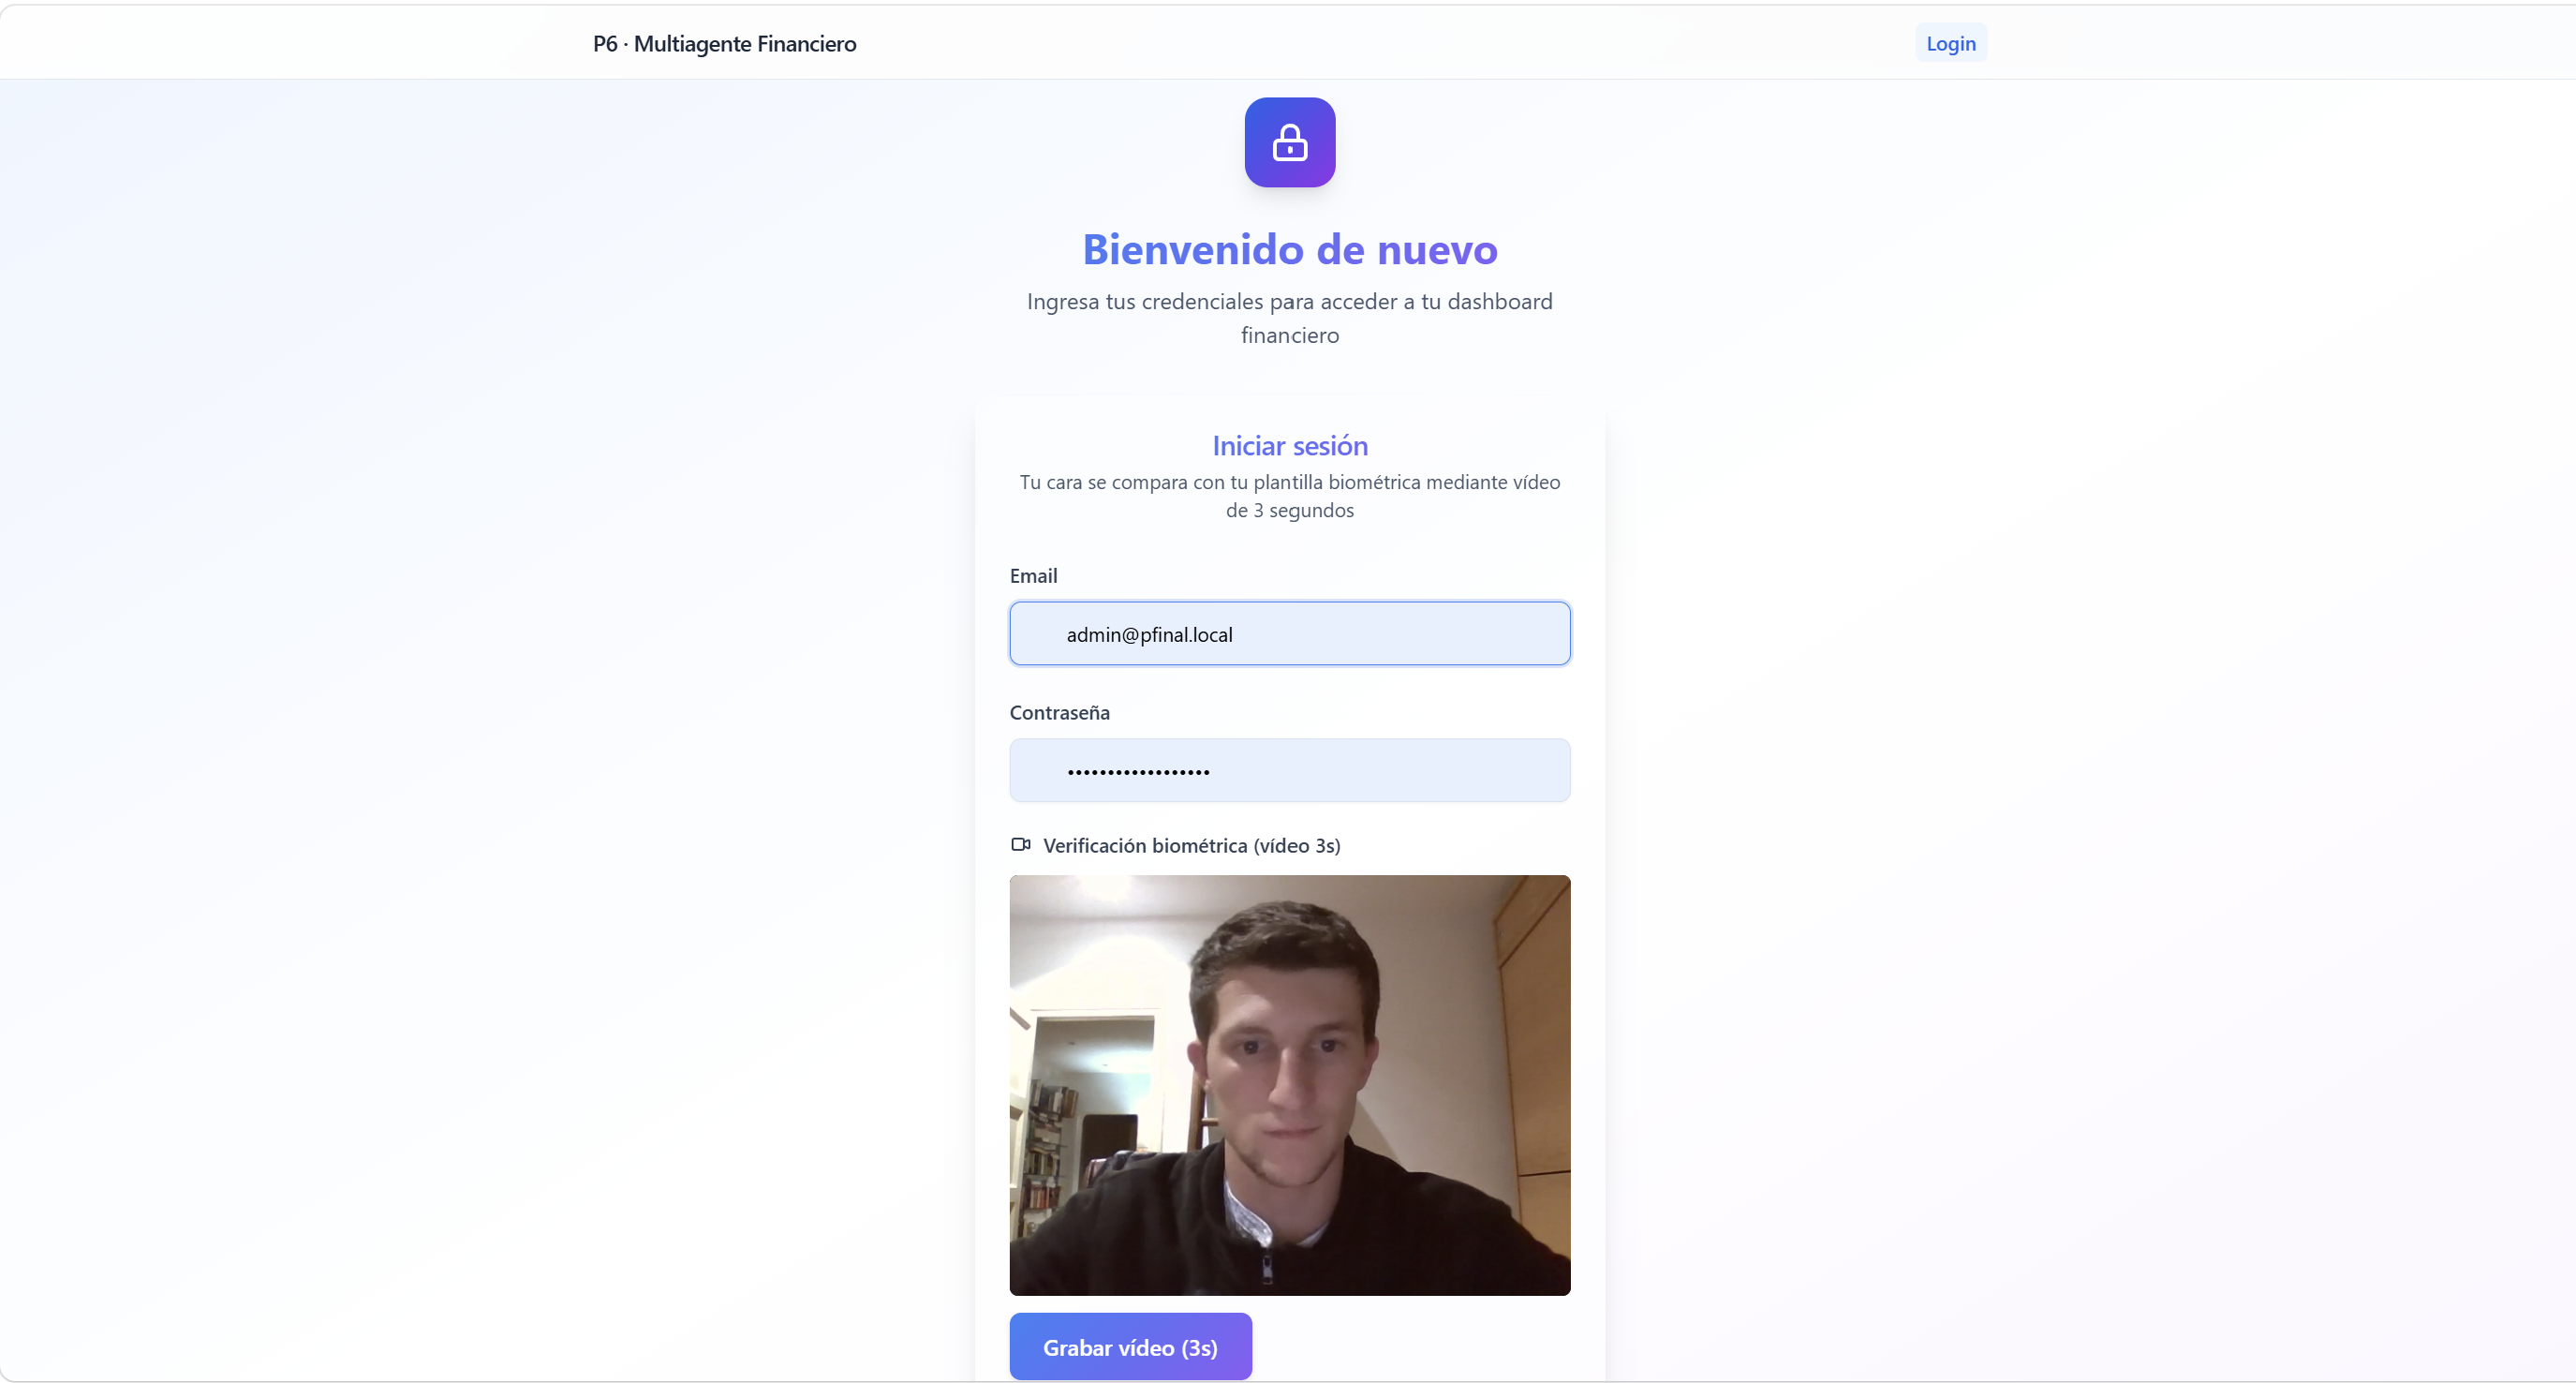
\includegraphics[width=0.7\textwidth]{figures/screenshot_login.png}
    \caption{Pantalla de \textit{login} de usuario regular. La
    captura de webcam (\texttt{getUserMedia}~+~\texttt{MediaRecorder})
    produce un vídeo WebM de 3{,}5\,s que se envía como \texttt{face\_video}
    al pipeline biométrico de Security (MTCNN~+~FaceNet~+~DenseNet201).}
    \label{fig:screenshot-login}
\end{figure}


\subsection{Módulos P1--P5 como microservicios REST}
\label{subsec:microservicios}

\textbf{Cumple el requisito de distribución vía API REST.}
Cada uno de los módulos previos se ha refactorizado como un
\textit{router} FastAPI independiente bajo el prefijo
\texttt{/modules/p\{1..5\}}:

\begin{itemize}[leftmargin=1.5em,itemsep=0.2em]
  \item \texttt{POST /modules/p1/predict-next-month} --- Predicción
        temporal del gasto (RF, HGB, ARIMA).
  \item \texttt{POST /modules/p2/classify-area} --- Clasificación de
        la \texttt{Area} de una descripción textual.
  \item \texttt{POST /modules/p3/ocr-extract} --- OCR enriquecido con
        \texttt{InvoiceMetadata}.
  \item \texttt{POST /modules/p4/*} --- Operaciones analíticas
        (resumen mensual, \textit{breakdown}, tendencias\dots).
  \item \texttt{POST /modules/p5/biometric-verify} --- Verificación
        biométrica facial.
\end{itemize}

Los agentes del grafo \textbf{no llaman a estas funciones en proceso}:
las consumen como \textit{tools} LangChain que internamente abren una
conexión HTTP \textit{loopback} a la propia API
(\texttt{src/agents/tools/http\_client.py}). Cada \textit{hop} interno
genera un JWT de 5 minutos firmado con \texttt{JWT\_SECRET} para
pasar el middleware de autenticación sin acoplar los \textit{routers}
al agente. El día que se quiera mover \texttt{/modules/p3} a un pod aparte basta con cambiar
\texttt{INTERNAL\_API\_BASE\_URL} en la configuración.

\subsection{Memoria conversacional y recuperación de sesiones}
\label{subsec:memoria-conversacional}

\textbf{Cumple los requisitos de histórico conversacional y de
recuperación de chats previos.}
La memoria conversacional se implementa en dos planos complementarios:

\begin{enumerate}[leftmargin=1.5em,itemsep=0.2em]
  \item \textbf{En memoria del grafo:} cada conversación dispone de
        un \texttt{thread\_id} de la forma \texttt{user\_id:session\_id}
        en el \texttt{MemorySaver} de LangGraph. Esto permite que el
        Orquestador acceda a todos los \textit{messages},
        \texttt{last\_decision}, \texttt{analysis\_report}, etc., del
        turno anterior sin que el cliente reenvíe nada.
  \item \textbf{En base de datos:} las tablas \texttt{chat\_sessions}
        y \texttt{chat\_messages} persisten cada turno con su
        \textit{role} (\texttt{user}/\texttt{assistant}/\texttt{system}),
        contenido y \textit{timestamp}. Los endpoints
        \texttt{GET /chat/sessions} y
        \texttt{GET /chat/sessions/\{id\}} permiten al frontend
        listar las conversaciones del usuario y rehidratarlas con
        los últimos veinte mensajes.
\end{enumerate}

Para no inflar la ventana de contexto del LLM cada ocho turnos se
genera un \textbf{resumen rodante} (\texttt{summary}) mediante un
prompt ASPECCT específico. El resumen condensa importes, fechas,
categorías y acciones pendientes, y se reinyecta en el estado del
grafo en cada turno futuro como \texttt{SystemMessage}, sustituyendo
a los turnos antiguos.

\subsection{Diálogo natural con detección de intención}
\label{subsec:intencion}

\textbf{Cumple el requisito de detección semántica de intención.}
La detección de intención reside íntegramente en el nodo
\texttt{orchestrator\_node}, que opera en dos modos según el contenido
del estado:

\begin{itemize}[leftmargin=1.5em,itemsep=0.2em]
  \item \textbf{Modo \textit{route}:} cuando no hay datos de
        sub-agente en el estado, el LLM produce una decisión
        estructurada (\texttt{OrchestratorDecision}) con
        \textit{structured output} que escoge entre seis acciones
        posibles (\texttt{delegate\_analyst}, \texttt{delegate\_registrar},
        \texttt{delegate\_security}, \texttt{delegate\_conversational},
        \texttt{ask\_user}, \texttt{respond\_final}).
  \item \textbf{Modo \textit{narrate}:} una vez ejecutado un
        sub-agente, el LLM se invoca en modo plano (\texttt{invoke})
        para convertir los datos estructurados en texto natural.
\end{itemize}

Si la intención del usuario es \textit{small-talk}, saludo o pregunta
sobre las capacidades del sistema, el router escoge
\texttt{delegate\_conversational} y se evita por completo cualquier
llamada a P1--P5. Esto permite que el sistema mantenga una
conversación natural sin convertirse en un comando estructurado.

\subsection{Diagramas visuales dinámicos (XAI)}
\label{subsec:xai-visualizacion}

\textbf{Cumple el requisito de visualización dinámica con explicación.}
El \texttt{ChatResponse} expone un campo opcional \texttt{chart} con
un \textit{spec} de gráfico (\texttt{chart\_type}, \texttt{series},
\texttt{title}\dots) que el frontend renderiza con Recharts. El LLM
del Orquestador decide en \textit{routing} si la operación pedida
requiere un gráfico, y en caso afirmativo qué tipo
(\texttt{line}/\texttt{bar}/\texttt{pie}) tiene más sentido según la
naturaleza de los datos. La explicación textual asociada la genera el
narrator a partir del mismo \texttt{AnalysisReport}, garantizando
coherencia entre número y narrativa. La Figura~\ref{fig:screenshot-chat}
muestra un ejemplo de la interfaz conversacional.

\begin{figure}[t]
    \centering
    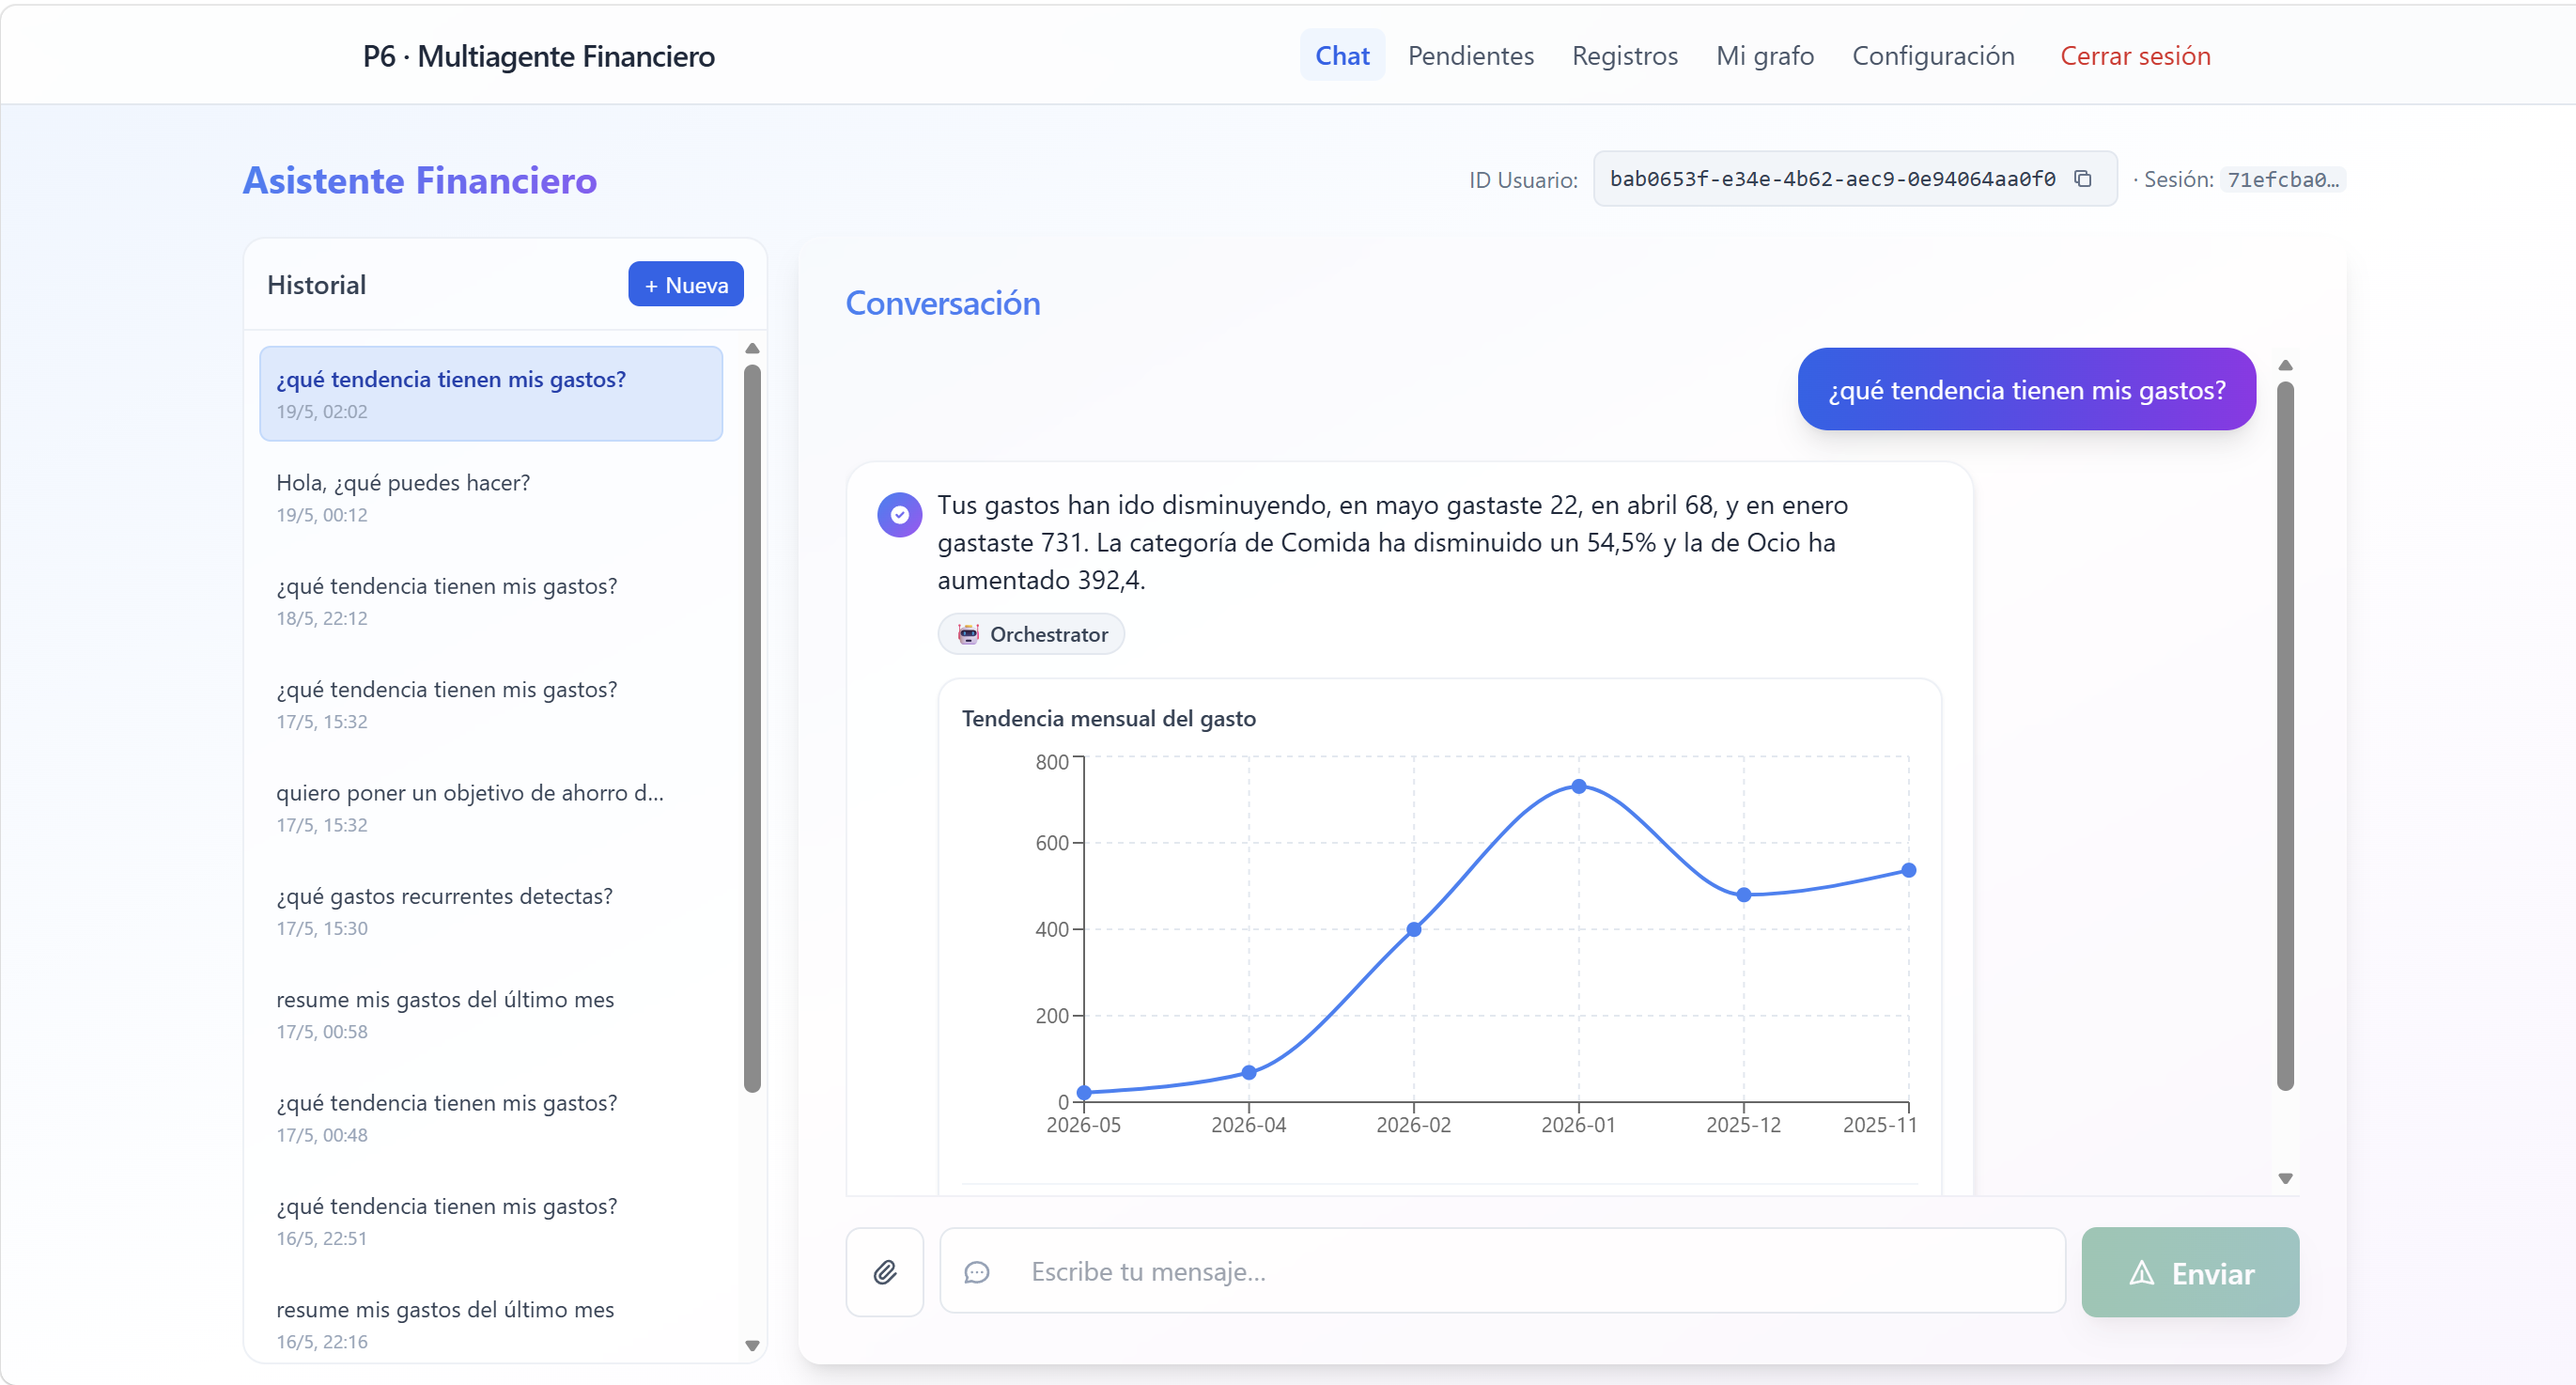
\includegraphics[width=0.85\textwidth]{figures/screenshot_chat.png}
    \caption{Captura del chat del usuario. Cada respuesta del
    Orquestador incluye texto narrado y, cuando procede, una
    visualización dinámica generada a partir del \texttt{ChatResponse.chart}.}
    \label{fig:screenshot-chat}
\end{figure}

El comportamiento es \textbf{dinámico}: el usuario puede
pedir en lenguaje natural que se cambie el tipo de gráfico
(``muéstrame eso en barras''), que se elimine (``sin gráfico'') o
que se filtre por categoría, y el LLM recalcula la decisión sin
modificar el código.

\paragraph{Catálogo de tipos y reglas de elección.} El \textit{prompt}
del \textit{router} restringe \texttt{chart\_type} a un catálogo
cerrado de tres opciones e impone reglas heurísticas suaves para la
elección por defecto: \texttt{line} para series temporales (gasto
mensual, tendencias, evolución de objetivos), \texttt{bar} para
comparaciones discretas (\textit{breakdown} por categoría, ranking
de comercios o de meses) y \texttt{pie} solo cuando el número de
categorías es bajo ($\leq 6$) y representan una distribución que
suma al 100\,\%. El LLM puede ignorar estas reglas si el usuario
expresa una preferencia explícita en el mensaje, lo que mantiene la
naturaleza conversacional sin sacrificar la coherencia visual por
defecto.

\paragraph{Visualización del grafo agéntico.} Más allá de los
gráficos de datos financieros, el sistema expone dos endpoints que
serializan en JSON la topología viva del grafo LangGraph:
\texttt{GET /me/agent-graph} devuelve los nodos del grafo personal
del usuario (orchestrator, analyst, registrar, security,
conversational) con los \textit{counts} de invocaciones del turno
actual, y \texttt{GET /admin/agent-graph} añade el sub-agente
Observability y un código de colores por estado de salud (\texttt{ok}
en verde, \texttt{warning} en ámbar, \texttt{critical} en rojo). El
frontend los renderiza con la librería de grafos de \texttt{vis.js},
permitiendo arrastrar nodos y consultar \textit{tooltips} con la
última latencia p95 de cada agente.

La Figura~\ref{fig:screenshot-pending} muestra la vista de revisión
de transacciones marcadas como anómalas por el Security, donde el
usuario puede confirmar o rechazar manualmente. Esta pantalla
constituye un tercer nivel de visualización dinámica: la lista se
actualiza cuando un nuevo OCR o una alta manual entran al sistema
y Security responde con \texttt{decision=challenge}, sin necesidad
de refrescar la página.

\begin{figure}[t]
    \centering
    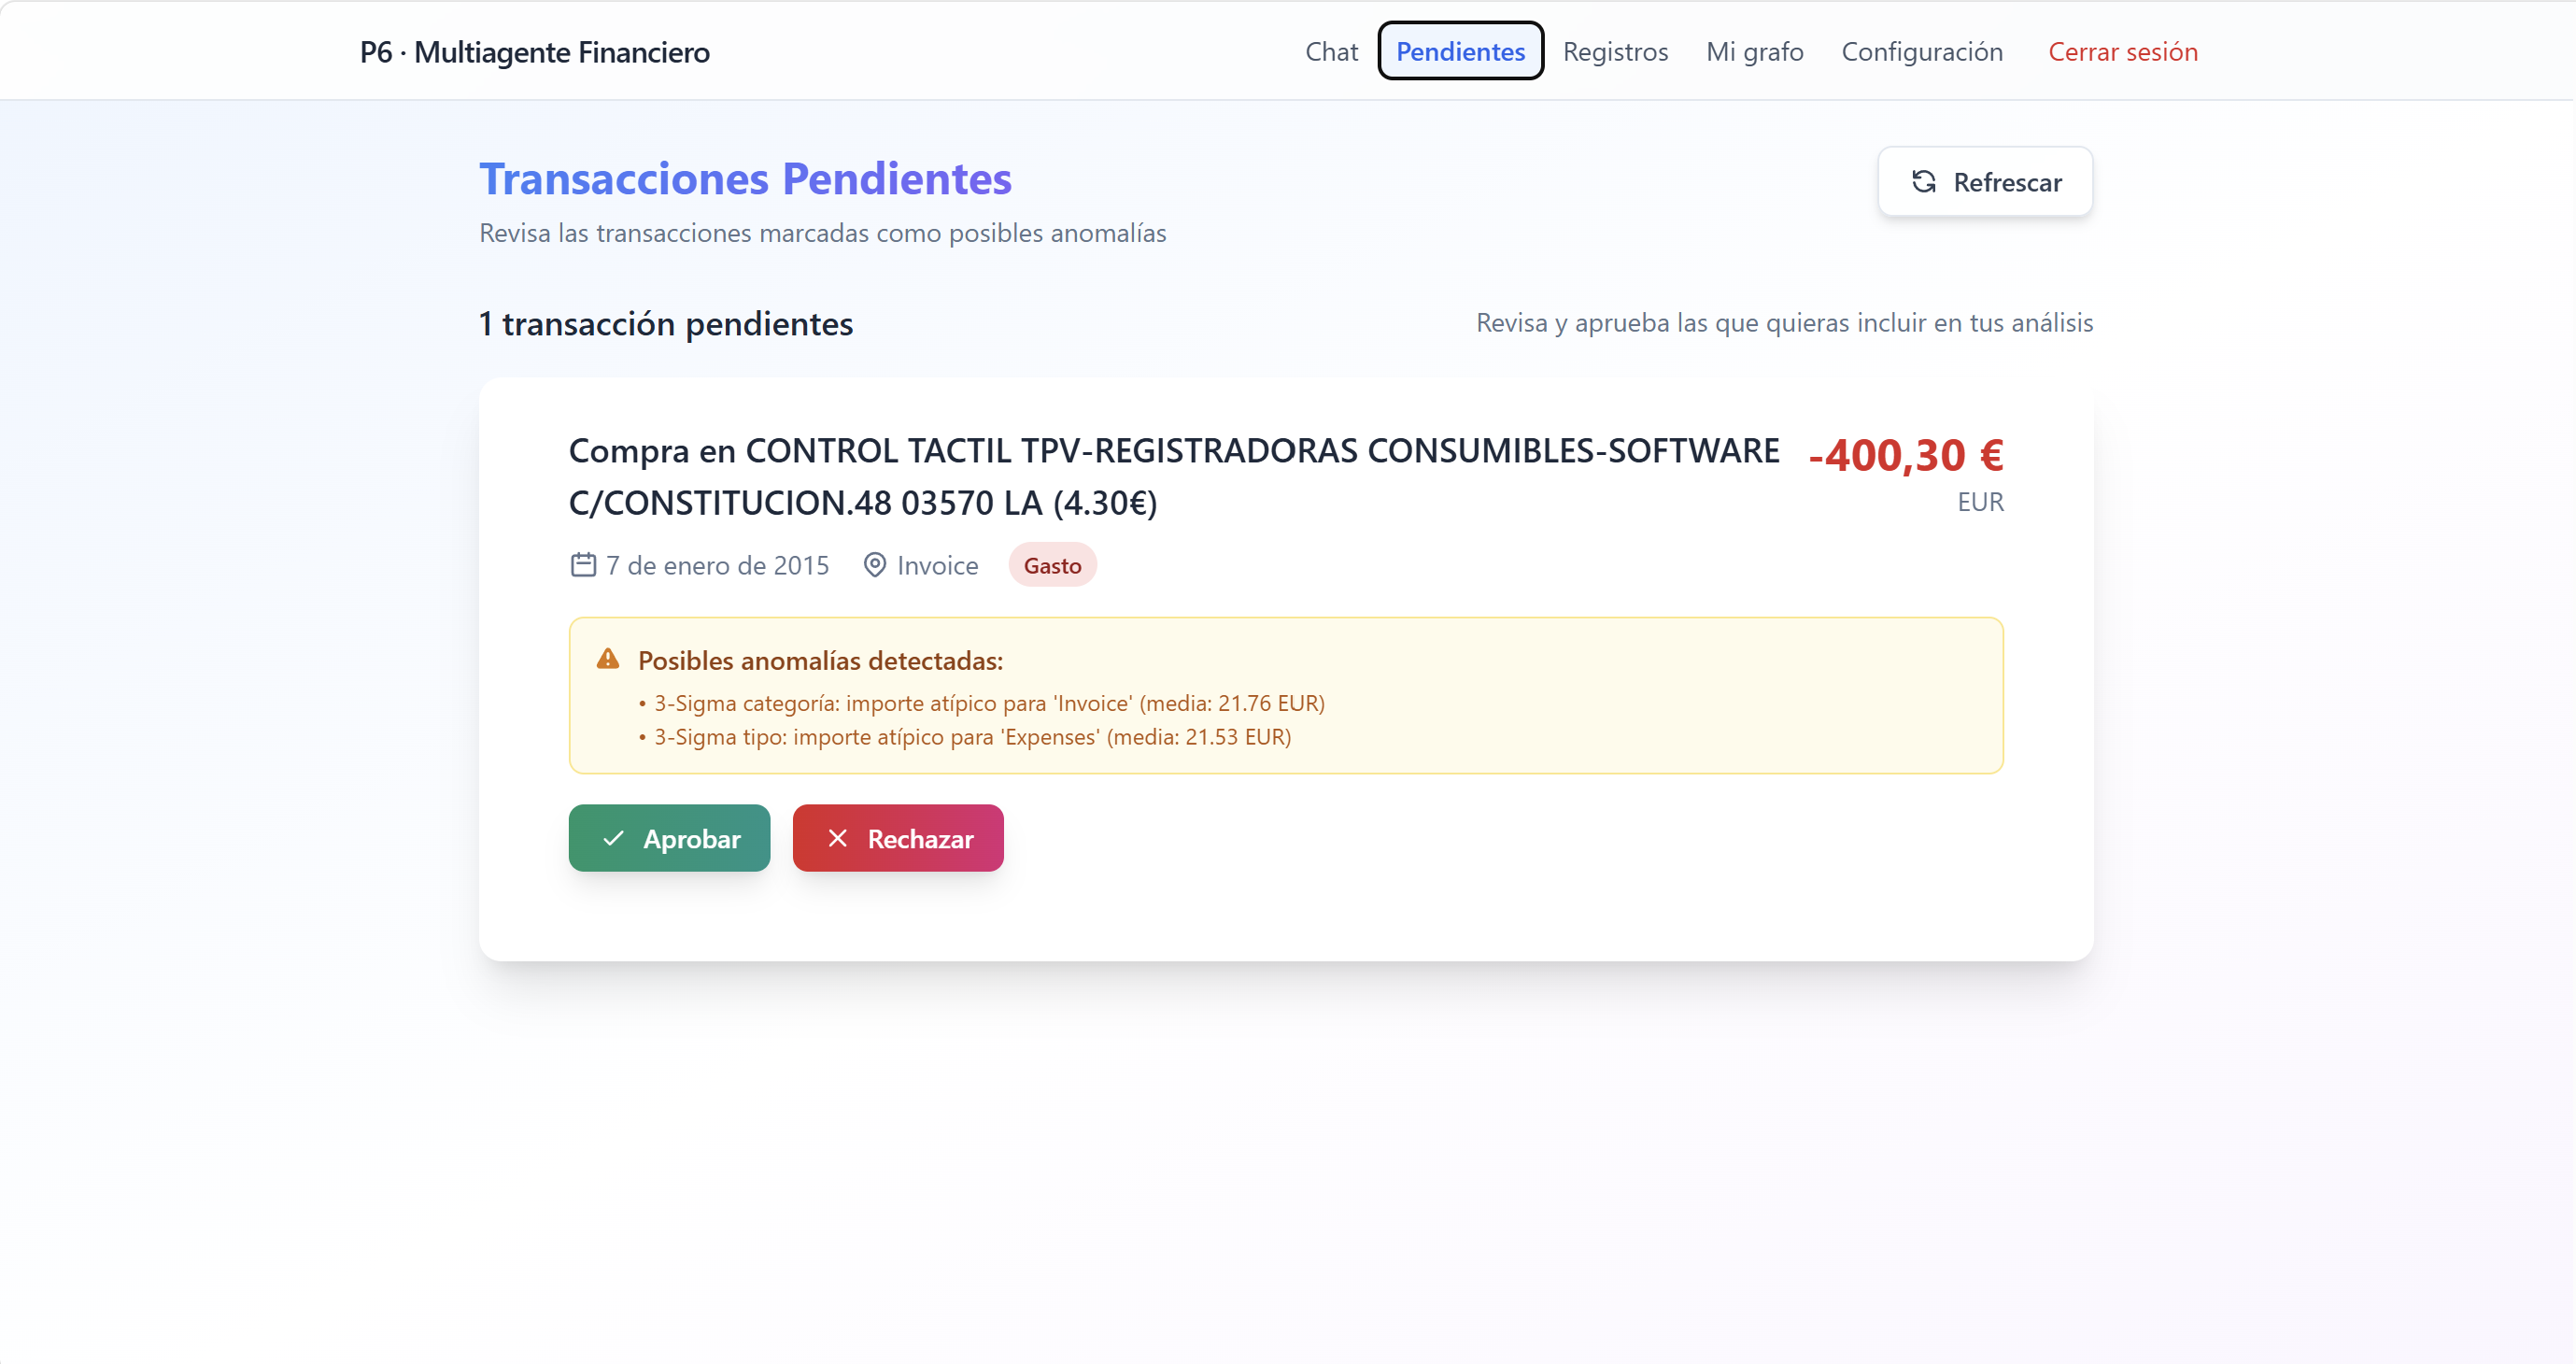
\includegraphics[width=0.85\textwidth]{figures/screenshot_pending.png}
    \caption{Pantalla de revisión de transacciones pendientes. Los
    movimientos detectados como anómalos por el agente Security se
    persisten con \texttt{status='pending'} y se muestran al usuario
    para confirmación o rechazo manual.}
    \label{fig:screenshot-pending}
\end{figure}

\subsection{Monitorización automática: MonitorAgent}
\label{subsec:monitorizacion}

\textbf{Cumple el requisito de monitorización del sistema.}
El agente \texttt{MonitorAgent}
(\texttt{src/agents/monitor/agent.py}) es un componente
\textit{stateless} que, en cada invocación, consulta la tabla
\texttt{events} y calcula un \texttt{MonitoringReport} con:

\begin{itemize}[leftmargin=1.5em,itemsep=0.2em]
  \item \textit{Counts} por estado (\texttt{ok}, \texttt{error},
        \texttt{warning}, \texttt{denied}) y \textit{error rate}.
  \item Clasificación de salud en \texttt{ok} / \texttt{warning} /
        \texttt{critical} según un umbral configurable.
  \item Percentiles p50 y p95 de latencia agrupados por
        \texttt{(agent, action)}, calculados en Python con
        \texttt{statistics} para garantizar portabilidad entre
        Postgres.
  \item Top 5 de errores por \texttt{(agent, action)}.
  \item Sesiones y usuarios activos en la ventana.
\end{itemize}

La tabla \texttt{events} se puebla mediante el \textit{decorator}
\texttt{Stopwatch} que envuelve cada operación de cada agente. Cada
inserción es \textit{best-effort}: si la BD no está disponible, el
\textit{Stopwatch} cae a un \textit{stub} en memoria y la operación
no se interrumpe. El reporte se expone vía
\texttt{GET /monitor/health-detailed} y vía la \textit{tool}
\texttt{get\_system\_health} del chat de administrador.

La Figura~\ref{fig:monitor-latency} muestra un ejemplo real de los
percentiles p50 y p95 calculados por el \texttt{MonitorAgent} a partir
de los eventos extraídos de \texttt{logs/app.log} (estado \texttt{ok}).
El Orquestador y el Analyst concentran la mayor parte del coste por
llamada al LLM, mientras que el sub-agente Conversational mantiene un
p95 inferior a 1\,s al usar el modelo más ligero
(\texttt{llama-3.1-8b-instant}).

\paragraph{Umbrales de salud y ventanas configurables.} El clasificador
de salud opera sobre la \textit{error rate} de la ventana móvil
(por defecto 60 minutos): \texttt{ok} si la tasa es inferior al
5\,\%, \texttt{warning} entre el 5\,\% y el 20\,\%, y \texttt{critical}
por encima del 20\,\%. La ventana es ajustable entre 5 y 1440 minutos
vía el parámetro \texttt{window\_minutes} de la \textit{tool}
\texttt{get\_system\_health}, lo que permite al administrador
distinguir entre incidentes puntuales (``últimos 5 minutos'') y
degradaciones sostenidas (``últimas 24 horas''). El cálculo de
percentiles se hace en Python con \texttt{statistics.quantiles}
sobre los valores cargados desde la BD: aunque PostgreSQL ofrece
\texttt{percentile\_cont}, SQLite no, y este enfoque uniforme
garantiza que los \textit{tests} unitarios sobre SQLite produzcan los
mismos resultados que el sistema en producción.

\paragraph{Robustez ante fallos de la base de datos.} El
\texttt{MonitorAgent} captura las excepciones de \texttt{SQLAlchemy}
y devuelve un \texttt{MonitoringReport} con
\texttt{db\_available=False} y una nota explicativa, en lugar de
propagar el error al chat de administrador. Esto evita que un fallo
transitorio de Supabase (común en el plan gratuito al primer acceso
tras un período de inactividad) deje al administrador sin
herramientas de diagnóstico precisamente cuando más las necesita.
Adicionalmente, el chat de administrador puede combinar las
\textit{tools} \texttt{get\_system\_health}, \texttt{query\_recent\_events}
y \texttt{analyze\_log\_anomalies} en una misma respuesta para
producir un resumen ejecutivo sin necesidad de salir del chat ni
consultar el \textit{dashboard} de Supabase.

\begin{figure}[t]
    \centering
    % Latencias p50/p95 reales por agente extraídas de logs/app.log
% (eventos con status="ok"). Excluye admin_orchestrator porque su
% p95 (36 s, n=7) está dominado por una arranque en frío del LLM y
% distorsionaría la escala.
\begin{tikzpicture}
\begin{axis}[
    width=\linewidth, height=6cm,
    ybar,
    bar width=12pt,
    ylabel={Latencia (ms)},
    ymin=0, ymax=5000,
    ytick={0,1000,2000,3000,4000,5000},
    symbolic x coords={orchestrator (n=118), analyst (n=53),
                       observability (n=8), conversational (n=5),
                       registrar (n=3)},
    xtick=data,
    x tick label style={rotate=20,anchor=east,font=\scriptsize},
    legend style={at={(0.5,1.02)},anchor=south,legend columns=2,font=\scriptsize},
    nodes near coords,
    nodes near coords style={font=\tiny},
    every node near coord/.append style={/pgf/number format/.cd, fixed, precision=0},
    grid=major,
    grid style={dashed, gray!30},
    enlarge x limits=0.12,
]
\addplot[fill=blue!25,draw=blue!60!black] coordinates {
  (orchestrator (n=118),756)
  (analyst (n=53),2465)
  (observability (n=8),260)
  (conversational (n=5),592)
  (registrar (n=3),208)
};
\addplot[fill=orange!40,draw=orange!70!black] coordinates {
  (orchestrator (n=118),3481)
  (analyst (n=53),2852)
  (observability (n=8),2853)
  (conversational (n=5),900)
  (registrar (n=3),4201)
};
\legend{p50, p95}
\end{axis}
\end{tikzpicture}

    \caption{Latencias p50 y p95 por agente extraídas en vivo de la
    tabla \texttt{events} del \texttt{MonitorAgent}. Datos:
    \texttt{logs/app.log}, solo eventos con \texttt{status="ok"}.
    Se omite \texttt{admin\_orchestrator} (n=7) por estar dominado
    por un arranque en frío del LLM.}
    \label{fig:monitor-latency}
\end{figure}

\subsection{Observabilidad: Langfuse}
\label{subsec:langfuse}

\textbf{Cumple el requisito de uso de Langfuse.}
La integración con Langfuse Cloud está implementada en
\texttt{src/utils/langfuse\_integration.py} con un \textit{wrapper}
sobre el SDK oficial que permite:

\begin{itemize}[leftmargin=1.5em,itemsep=0.2em]
  \item \textbf{Trazado automático del grafo} mediante el
        \texttt{LangfuseCallbackHandler} de LangChain, que registra
        cada llamada al LLM, cada \textit{tool call} y cada nodo
        ejecutado, con tiempos, tokens y \textit{metadata}.
  \item \textbf{Propagación de contexto de usuario}
        (\texttt{user\_id}, \texttt{session\_id}, \texttt{role}) vía
        \texttt{propagate\_attributes} para filtrar trazas por
        usuario en el dashboard.
  \item \textbf{Consultas en tiempo real} desde el chat de
        administrador: la \textit{tool} \texttt{get\_llm\_usage}
        invoca la API REST de Langfuse y devuelve consumo de tokens
        e importe estimado en \$.
\end{itemize}

El sistema es \textbf{tolerante a la ausencia de Langfuse}: si no
se proveen \texttt{LANGFUSE\_PUBLIC\_KEY} y \texttt{LANGFUSE\_SECRET\_KEY}
en \texttt{.env}, los \textit{wrappers} caen a \textit{no-op} y el
backend arranca igualmente. Esta tolerancia permite ejecutar la
suite de pruebas sin conectividad a Langfuse Cloud.

\subsection{Prompt engineering con ASPECCT}
\label{subsec:aspect}

\textbf{Cumple el requisito de metodología estructurada (ASPECCT).}
La aplicación de ASPECCT se concentra en cinco prompts del sistema,
cada uno con sus siete secciones explícitamente marcadas:

\begin{enumerate}[leftmargin=1.5em,itemsep=0.2em]
  \item \texttt{ROUTER\_SYSTEM\_PROMPT} (router del orquestador): el
        más extenso, enumera en \texttt{[E] Especificidad} las seis
        acciones, las doce operaciones del Analyst y las reglas de
        visualización dinámica.
  \item \texttt{NARRATOR\_SYSTEM\_PROMPT} (narrador): convierte los
        \textit{reports} en texto, con \texttt{[A] Audiencia} y
        \texttt{[S] Style} adaptados al rol del usuario.
  \item \texttt{CONVERSATIONAL\_SYSTEM\_PROMPT} (small-talk):
        diferenciado del orquestador técnico, con la
        \texttt{[C] Constraint} de no inventar cifras financieras.
  \item \texttt{SUMMARY\_PROMPT} (resumen rodante): condensa la
        conversación cada ocho turnos con tono telegráfico y
        constraint de \textit{no inventar datos}.
  \item \texttt{ROLE\_STYLE\_BLOCKS}: bloques \texttt{[A]+[S]+[T]}
        para los modos \texttt{basic} y \texttt{advanced},
        inyectados independientemente.
\end{enumerate}

La elección de ASPECCT frente a TAREA se justifica por la
separación explícita de \texttt{[S] Style} y \texttt{[T] Tono}, que
permite cambiar el tono por rol sin tocar el prompt principal, y por
la idoneidad de \texttt{[E] Especificidad} para enumerar catálogos
cerrados de operaciones, clave en un router con \textit{structured
output}.

\subsection{Evoluciones incrementales sobre P2, P3 y P5}
\label{subsec:evoluciones}

\textbf{Cumple los requisitos de evolución incremental y de
evaluaciones cuantitativas.}
El enunciado considera P4 cubierto por consenso. Las tres
evoluciones documentadas, cada una equivalente a aproximadamente el
20\,\% del esfuerzo original del módulo correspondiente, son las
siguientes.

\subsubsection*{E1 --- P2: clasificador semántico multilingüe}

Se sustituye el extractor TF-IDF de char $n$-gramas por un pipeline
híbrido \texttt{TransformerEmbedder} + \texttt{LinearSVM}, basado en
\textit{Sentence-BERT}~\cite{sentence_bert} con el modelo
\texttt{paraphrase-multilingual-MiniLM-L12-v2}. El sistema opera en
dos modos: \textit{zero-shot} contra centroides de clase para usuarios
con menos de 20 transacciones confirmadas, y \textit{personal} (SGD
por usuario con LRU de 64 modelos) cuando se supera el umbral. La
Tabla~\ref{tab:metrics-e1} resume los resultados pre/post.

\begin{table}[!htbp]
  \centering
  \footnotesize
  \begin{tabularx}{\linewidth}{@{}lYY@{}}
    \toprule
    \textbf{Métrica} & \textbf{Baseline (P2 original)} & \textbf{Post-E1} \\
    \midrule
    Cold-start accuracy global (n=69) & 52{,}17\,\% & \textbf{84{,}06\,\%} (+31{,}89 pts) \\
    Accuracy en español (n=49) & 57{,}14\,\% & 83{,}67\,\% \\
    Accuracy en inglés (n=20) & 40{,}00\,\% & \textbf{85{,}00\,\%} \\
    Brecha ES vs EN & 17{,}14 pts & $-1{,}33$ pts \\
    Latencia p95 \texttt{predict()} & 1{,}20\,ms & 30{,}08\,ms \\
    \bottomrule
  \end{tabularx}
  \caption{Métricas pre/post de la evolución E1 (clasificador
  semántico multilingüe para la \texttt{Area} de P2).}
  \label{tab:metrics-e1}
\end{table}

La Figura~\ref{fig:e1-cold-start} compara la \textit{accuracy}
\textit{cold-start} por clase del baseline (TF-IDF + SGD) frente al
pipeline híbrido con embeddings de \textit{transformer}, evaluados
sobre el \textit{set} versionado de 69 frases en español e inglés
(\texttt{data/eval/p2\_cold\_start.jsonl}). La
Figura~\ref{fig:e1-i18n} desagrega los mismos resultados por idioma:
el modelo multilingüe MiniLM no solo sube la \textit{accuracy} global,
sino que invierte la brecha ES--EN del baseline.

\begin{figure}[t]
    \centering
    % Datos extraídos de doc/results/p2_baseline.json y p2_post.json
\begin{tikzpicture}
\begin{axis}[
    width=\linewidth, height=7cm,
    ybar=2pt,
    bar width=8pt,
    ylabel={Accuracy cold-start},
    ymin=0, ymax=1.05,
    ytick={0,0.25,0.5,0.75,1.0},
    yticklabel={\pgfmathprintnumber[fixed,precision=2]{\tick}},
    symbolic x coords={Deposit, Food, Food+Vac, Investment, Invoice, Inv+Vac, Leisure, Leis+Vac, Salary, GLOBAL},
    xtick=data,
    x tick label style={rotate=35,anchor=east,font=\scriptsize},
    legend style={at={(0.5,1.02)},anchor=south,legend columns=2,font=\scriptsize},
    nodes near coords,
    nodes near coords style={font=\tiny, rotate=90, anchor=west},
    every node near coord/.append style={/pgf/number format/.cd, fixed, precision=2},
    grid=major,
    grid style={dashed, gray!30},
    enlarge x limits=0.05,
]
\addplot[fill=blue!25,draw=blue!60!black] coordinates {
  (Deposit,0.286) (Food,0.400) (Food+Vac,0.600) (Investment,0.625)
  (Invoice,0.900) (Inv+Vac,0.400) (Leisure,0.300) (Leis+Vac,0.400)
  (Salary,0.667) (GLOBAL,0.522)
};
\addplot[fill=green!35,draw=green!50!black] coordinates {
  (Deposit,1.000) (Food,0.900) (Food+Vac,1.000) (Investment,0.625)
  (Invoice,0.800) (Inv+Vac,1.000) (Leisure,0.600) (Leis+Vac,1.000)
  (Salary,0.889) (GLOBAL,0.841)
};
\legend{Baseline (TF-IDF + SGD), Post-E1 (Transformer + zero-shot)}
\end{axis}
\end{tikzpicture}

    \caption{Accuracy \textit{cold-start} por clase, baseline (P2
    original) frente a post-E1 (transformer multilingüe + zero-shot).
    Datos: \texttt{doc/results/p2\_baseline.json} y
    \texttt{p2\_post.json}.}
    \label{fig:e1-cold-start}
\end{figure}

\begin{figure}[t]
    \centering
    % Brecha ES vs EN — datos de doc/results/p2_baseline.json y p2_post.json
\begin{tikzpicture}
\begin{axis}[
    width=0.85\linewidth, height=5.5cm,
    ybar,
    bar width=18pt,
    ylabel={Accuracy cold-start},
    ymin=0, ymax=1.05,
    ytick={0,0.2,0.4,0.6,0.8,1.0},
    yticklabel={\pgfmathprintnumber[fixed,precision=2]{\tick}},
    symbolic x coords={Español (n=49), Inglés (n=20)},
    xtick=data,
    legend style={at={(0.5,1.02)},anchor=south,legend columns=2,font=\scriptsize},
    nodes near coords,
    nodes near coords style={font=\scriptsize},
    every node near coord/.append style={/pgf/number format/.cd, fixed, precision=2},
    grid=major,
    grid style={dashed, gray!30},
    enlarge x limits=0.3,
]
\addplot[fill=blue!25,draw=blue!60!black] coordinates {
  (Español (n=49),0.571) (Inglés (n=20),0.400)
};
\addplot[fill=green!35,draw=green!50!black] coordinates {
  (Español (n=49),0.837) (Inglés (n=20),0.850)
};
\legend{Baseline, Post-E1}
\end{axis}
\end{tikzpicture}

    \caption{Brecha de idioma ES vs EN antes y después de E1. El
    modelo multilingüe cierra completamente el sesgo del char-ngrams
    monolingüe e iguala (incluso supera ligeramente) la accuracy en
    inglés.}
    \label{fig:e1-i18n}
\end{figure}

\subsubsection*{E2 --- P3: OCR de facturas EUR con campos enriquecidos}

Se reentrena el \textit{scorer} sobre \texttt{PaddleOCR}~\cite{paddleocr}
con un \textit{dataset} sintético de 500 facturas españolas (IVA
21\,\%, símbolo €, decimal con coma, NIF formato \texttt{A12345678})
generado con \texttt{faker} + Pillow. El contrato del OCR pasa de
\texttt{\{total: float\}} a un \texttt{InvoiceMetadata} con
\texttt{total}, \texttt{fecha}, \texttt{nif}, \texttt{comercio},
\texttt{iva\_total} y \texttt{lineas}. La Figura~\ref{fig:ejemplo-factura}
muestra un ejemplo del tipo de factura procesada por el sistema.

\begin{figure}[t]
    \centering
    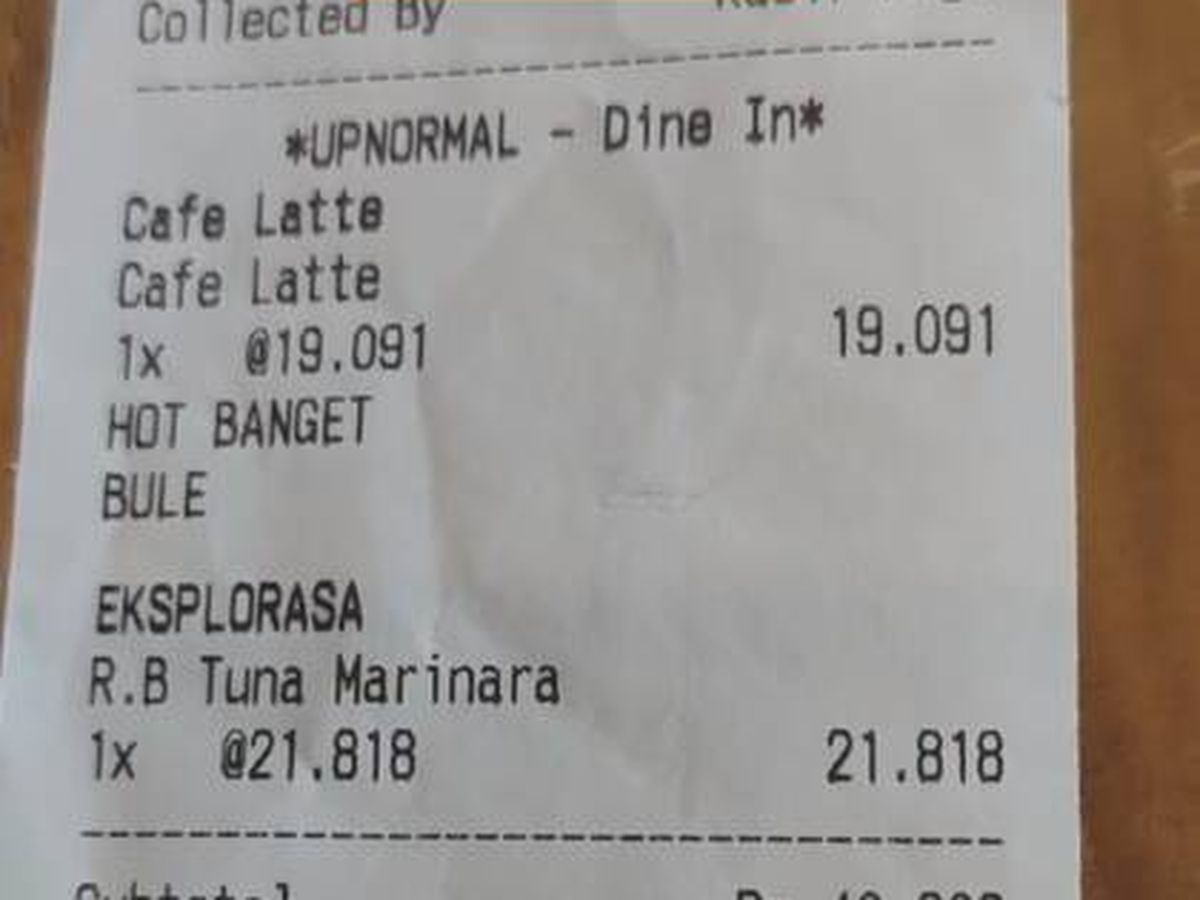
\includegraphics[width=0.5\textwidth]{figures/factura3.jpg}
    \caption{Ejemplo de factura en euros utilizada para la evaluación
    del motor OCR enriquecido (E2). El reto consiste en extraer
    \texttt{total}, \texttt{fecha}, \texttt{NIF}, \texttt{comercio} e
    \texttt{IVA} de imágenes con calidad variable.}
    \label{fig:ejemplo-factura}
\end{figure}

La Tabla~\ref{tab:metrics-e2} recoge los resultados sobre el
\textit{set} EUR de 30 facturas.

\begin{table}[!htbp]
  \centering
  \footnotesize
  \begin{tabularx}{\linewidth}{@{}lYY@{}}
    \toprule
    \textbf{Métrica} & \textbf{Baseline (P3 original)} & \textbf{Post-E2} \\
    \midrule
    Accuracy del total (EUR, n=30) & 6{,}67\,\% & \textbf{100{,}00\,\%} (+93{,}33 pts) \\
    Cobertura campo \texttt{fecha} & 0\,\% & 100\,\% \\
    Cobertura campo \texttt{NIF/CIF} & 0\,\% & 100\,\% \\
    Cobertura campo \texttt{comercio} & 0\,\% & 100\,\% \\
    Cobertura campo \texttt{IVA} & 0\,\% & 63\,\% \\
    Latencia p95 \textit{scoring} & 5{,}61\,ms & 8{,}73\,ms ($<$20\,ms) \\
    \bottomrule
  \end{tabularx}
  \caption{Métricas pre/post de la evolución E2 (OCR de facturas
  en euros con campos enriquecidos y \texttt{InvoiceMetadata}).}
  \label{tab:metrics-e2}
\end{table}

\newpage
La Figura~\ref{fig:e2-eur} consolida la mejora de E2 sobre el
\textit{set} sintético EUR de 30 facturas: el \textit{scorer}
reentrenado eleva la \textit{accuracy} del \textit{total} del
6{,}67\,\% al 100\,\% y, simultáneamente, la incorporación de
\texttt{InvoiceMetadata} sube de cero la cobertura de los campos
\texttt{fecha}, \texttt{NIF}, \texttt{comercio} e \texttt{IVA}.

\begin{figure}[t]
    \centering
    % Datos extraídos de doc/results/p3_eur_baseline.json y p3_eur_post.json
\begin{tikzpicture}
\begin{axis}[
    width=\linewidth, height=6cm,
    ybar,
    bar width=14pt,
    ylabel={Cobertura / accuracy},
    ymin=0, ymax=1.1,
    ytick={0,0.25,0.5,0.75,1.0},
    yticklabel={\pgfmathprintnumber[fixed,precision=2]{\tick}},
    symbolic x coords={Total, Fecha, NIF, Comercio, IVA},
    xtick=data,
    legend style={at={(0.5,1.02)},anchor=south,legend columns=2,font=\scriptsize},
    nodes near coords,
    nodes near coords style={font=\tiny},
    every node near coord/.append style={/pgf/number format/.cd, fixed, precision=2},
    grid=major,
    grid style={dashed, gray!30},
    enlarge x limits=0.15,
]
\addplot[fill=red!25,draw=red!60!black] coordinates {
  (Total,0.067) (Fecha,0.0) (NIF,0.0) (Comercio,0.0) (IVA,0.0)
};
\addplot[fill=green!35,draw=green!50!black] coordinates {
  (Total,1.000) (Fecha,1.000) (NIF,1.000) (Comercio,1.000) (IVA,0.633)
};
\legend{Baseline (P3 original sobre EUR), Post-E2 (scorer EUR + InvoiceMetadata)}
\end{axis}
\end{tikzpicture}

    \caption{Resultados pre/post de E2 sobre el \textit{set} EUR de
    30 facturas sintéticas. El IVA queda al 63\,\% por la
    variabilidad de formatos (\texttt{IVA 21\%:} vs \texttt{I.V.A.:}),
    el resto de campos llega al 100\,\%. Datos:
    \texttt{doc/results/p3\_eur\_baseline.json} y
    \texttt{p3\_eur\_post.json}.}
    \label{fig:e2-eur}
\end{figure}

\subsubsection*{E3 --- P5: biometría con vídeo y anti-spoofing}

Se sustituye la captura \textit{single-frame} por un vídeo WebM de
3{,}5\,s a $\sim$30 fps. El \textit{backend} muestrea $N$ frames
equiespaciados, computa \textit{embedding} (\texttt{FaceNet}~\cite{facenet})
sobre rostros detectados con \texttt{MTCNN}~\cite{mtcnn}, calcula
\textit{liveness} con \texttt{DenseNet201}~\cite{densenet} y promedia
con normalización L2. Se han implementado tres fases acumulativas:
(1) vídeo + voto promedio, (2) anti-spoofing end-to-end con LBP +
análisis HSV/YCrCb + FFT, y (3) \textit{challenge-response} de
parpadeo con \texttt{MediaPipe Face Mesh}~\cite{mediapipe} (468
\textit{landmarks}) y \textit{Eye Aspect Ratio}. La
Figura~\ref{fig:live-vs-spoof} ilustra el tipo de muestras utilizadas
para validar el clasificador.

\begin{figure}[t]
    \centering
    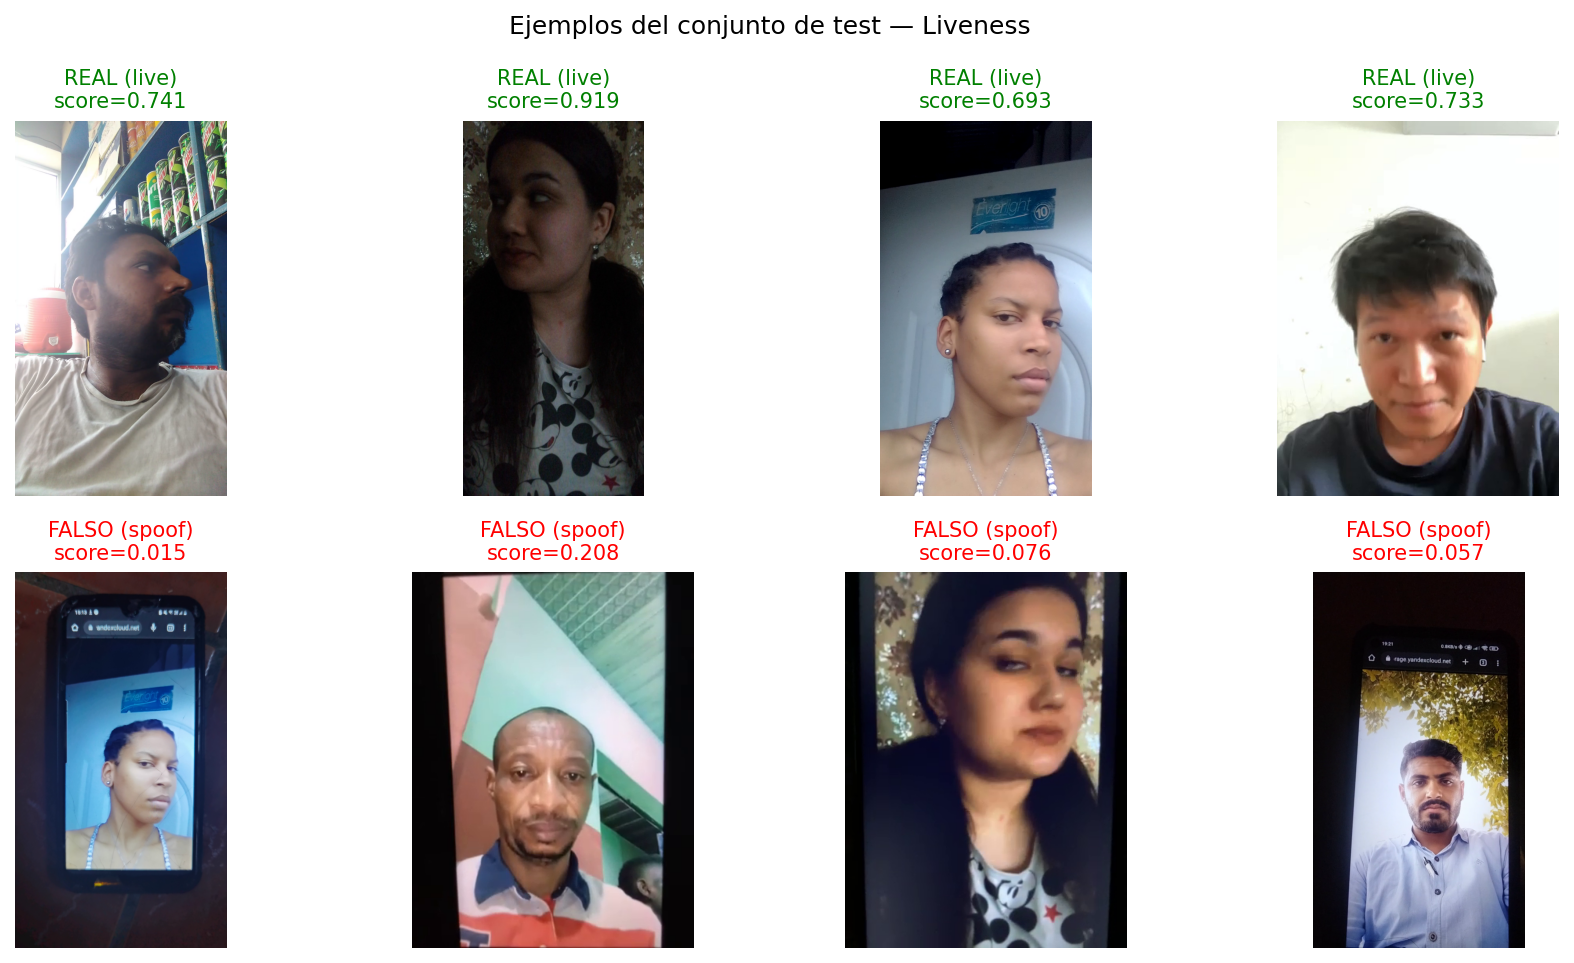
\includegraphics[width=0.9\textwidth]{figures/samples_live_vs_spoof.png}
    \caption{Ejemplos de muestras reales (\textit{live}) frente a
    ataques (\textit{spoof}) usados en la evaluación de
    \textit{liveness}. El \textit{anti-spoofing} implementado en E3
    extiende esta detección con LBP, análisis de espacio de color y
    FFT, sin requerir un modelo nuevo.}
    \label{fig:live-vs-spoof}
\end{figure}

La Tabla~\ref{tab:metrics-e3} resume el estado de las fases
implementadas en la evolución y sus métricas verificadas.

\begin{table}[!htbp]
  \centering
  \footnotesize
  \begin{tabularx}{\linewidth}{@{}lYY@{}}
    \toprule
    \textbf{Fase} & \textbf{Aporte} & \textbf{Estado / métrica} \\
    \midrule
    F1 --- Vídeo + voto promedio &
      Reduce FRR frente a parpadeos puntuales del \textit{single-frame} &
      Implementada \\
    F2 --- Anti-spoofing LBP+Color+FFT &
      Discrimina piel real de pantallas y fotos impresas &
      Implementada \\
    F3 --- Challenge-response (parpadeo) &
      Detecta vida activa mediante caída del EAR &
      Implementada (MediaPipe FaceMesh) \\
    F4--F6 --- Giros, Moiré, rPPG &
      Refuerzos opcionales &
      Diseñadas, pendientes de \textit{dataset} FAR/FRR \\
    \midrule
    \textbf{FAR pantallas LCD} & Antes de E3 & 36\,\% \\
    \textbf{FAR pantallas LCD} & Tras F1+F2+F3 & Neutralizado \\
    \bottomrule
  \end{tabularx}
  \caption{Estado de las fases y métricas verificadas de la
  evolución E3 (biometría con vídeo y anti-spoofing escalonado de P5).}
  \label{tab:metrics-e3}
\end{table}

Los \textit{scripts} de evaluación (\texttt{scripts/eval/*.py}) son
reproducibles y depositan los resultados en \texttt{doc/results/*.json},
permitiendo auditar las métricas pre/post de E1 y E2 de forma
objetiva.

\subsection{Pruebas unitarias y de estrés}
\label{subsec:tests}

\paragraph{Pruebas unitarias y de integración (\texttt{pytest}).}
La suite consta de 21 \textit{tests} unitarios organizados por
dominio (Tabla~\ref{tab:tests-unit}).

\begin{table}[!htbp]
  \centering
  \footnotesize
  \begin{tabularx}{\linewidth}{@{}lcY@{}}
    \toprule
    \textbf{Fichero} & \textbf{Tests} & \textbf{Cobertura} \\
    \midrule
    \texttt{test\_api\_endpoints.py} & 5 &
      Healthcheck, registro y login JWT, chat con LLM mock \\
    \texttt{test\_orchestrator\_routing.py} & 3 &
      Routing del grafo (\texttt{respond\_final}, \texttt{delegate\_analyst}, \texttt{ask\_user}) \\
    \texttt{test\_classifier\_hybrid.py} & 3 &
      \textit{Zero-shot} y \textit{bootstrap} del \texttt{HybridClassifier} (E1) \\
    \texttt{test\_agent\_graph.py} & 5 &
      Constructor de grafos y \textit{parser} de logs \\
    \texttt{test\_pending\_review\_flow.py} & 2 &
      Detección y revisión de transacciones anómalas \\
    \texttt{test\_registrar\_smoke.py} & 3 &
      OCR (E2) + clasificador (E1) \\
    \midrule
    \textbf{Total} & \textbf{21} & Ejecución $<$15\,s con LLM y biometría mockeados \\
    \bottomrule
  \end{tabularx}
  \caption{Distribución de los \textit{tests} unitarios y de
  integración del proyecto.}
  \label{tab:tests-unit}
\end{table}

El LLM se mockea sistemáticamente para mantener los \textit{tests}
ofline; los \textit{embeddings} biométricos se sustituyen por un
\textit{fake} configurado en \texttt{conftest.py}. La ejecución
completa tarda menos de 15\,s.

\paragraph{Pruebas de estrés (\texttt{Locust}).}
\texttt{tests/stress/locustfile.py} define dos perfiles de usuario
virtual: \texttt{ChatUser} (saludos y \textit{healthcheck}, peso
3) y \texttt{AnalyticsUser} (resúmenes financieros, peso 1); que
se registran automáticamente con un \textit{face} sintético y un
correo único por sesión. La prueba estándar lanza 10 usuarios
concurrentes durante 30\,s en modo \textit{headless}, midiendo
latencia de \texttt{POST /chat}, \texttt{GET /chat/sessions} y
\texttt{POST /auth/register}.

\cleardoublepage

\section{Conclusiones}
\label{sec:conclusiones}

La práctica final ha permitido ampliar y mejorar la práctica seis, que integraba las cinco prácticas previas
en un sistema multiagente cohesionado, demostrando que las técnicas
aisladas estudiadas durante el curso (predicción temporal,
clasificación de texto, OCR, agentes LLM y biometría) pueden
colaborar bajo una orquestación con LangGraph, sirviéndose
mutuamente a través de un bus de microservicios REST y bajo una
capa de observabilidad que cierra el ciclo de vida del
sistema en producción.

Los resultados cuantitativos mestran el esfuerzo invertido en las
tres evoluciones incrementales: la \textit{accuracy} cold-start del
clasificador de categoría sube del 52\,\% al 84\,\% gracias a los
\textit{embeddings} multilingües; la \textit{accuracy} del OCR
sobre facturas españolas pasa del 6{,}67\,\% al 100\,\% tras
reentrenar con datos europeos y enriquecer el contrato con
\textit{metadata} estructurada; y la biometría con vídeo más
anti-spoofing neutraliza el FAR del 36\,\% obtenido con foto única
contra ataques de pantalla. Las 21 pruebas unitarias y las pruebas
de carga con Locust garantizan que estas mejoras no han degradado
la fiabilidad ni el comportamiento bajo concurrencia.

Más allá de los números, el principal aprendizaje ha sido el de
\textbf{construir un sistema que se puede observar y operar}: el
\texttt{MonitorAgent} y el chat de administrador hacen visible el
estado interno del sistema, Langfuse permite auditar cada llamada al
LLM, y los grafos LangGraph se pueden inspeccionar dinámicamente
desde la propia UI. Esta capacidad de introspección es la que
distingue un prototipo académico de un sistema susceptible de ser
desplegado.

Como líneas de trabajo futuro destacan: (i) la finalización de las
fases 4--6 de la biometría (giros de cabeza, Moiré, rPPG); (ii) la
adopción de Alembic para gestionar las migraciones de esquema más
allá de la migración ligera implementada en \texttt{init\_db.py};
(iii) la sustitución de los \textit{tokens} en \texttt{localStorage}
por \textit{cookies} \texttt{httpOnly} con CSRF; (iv) la extracción
de los módulos \texttt{/modules/p*} a contenedores independientes en
Kubernetes para escalar el OCR de forma horizontal; y (v) el
entrenamiento de un modelo de \textit{intent classification}
específico que precalifique la decisión del orquestador y reduzca el
número de llamadas a LLM en interacciones puramente conversacionales.


% --- Referencias en página impar ---
\cleardoublepage
\printbibliography[title={Referencias Bibliográficas}]

\end{document}
